%% LyX 2.1.4 created this file.  For more info, see http://www.lyx.org/.
%% Do not edit unless you really know what you are doing.
\documentclass[oneside,english]{amsart}
\usepackage{lmodern}
\renewcommand{\sfdefault}{lmss}
\renewcommand{\ttdefault}{lmtt}
\usepackage[T1]{fontenc}
\usepackage[latin9]{inputenc}
\usepackage[letterpaper]{geometry}
\geometry{verbose}
\setcounter{secnumdepth}{2}
\setcounter{tocdepth}{2}
\setlength{\parskip}{\medskipamount}
\setlength{\parindent}{0pt}
\usepackage{color}
\usepackage{babel}
\usepackage{float}
\usepackage{amstext}
\usepackage{amsthm}
\usepackage{amssymb}
\usepackage{graphicx}
\usepackage{wasysym}
\usepackage[unicode=true,pdfusetitle,
 bookmarks=true,bookmarksnumbered=false,bookmarksopen=false,
 breaklinks=false,pdfborder={0 0 1},backref=false,colorlinks=true]
 {hyperref}

\makeatletter

%%%%%%%%%%%%%%%%%%%%%%%%%%%%%% LyX specific LaTeX commands.
%% Special footnote code from the package 'stblftnt.sty'
%% Author: Robin Fairbairns -- Last revised Dec 13 1996
\let\SF@@footnote\footnote
\def\footnote{\ifx\protect\@typeset@protect
    \expandafter\SF@@footnote
  \else
    \expandafter\SF@gobble@opt
  \fi
}
\expandafter\def\csname SF@gobble@opt \endcsname{\@ifnextchar[%]
  \SF@gobble@twobracket
  \@gobble
}
\edef\SF@gobble@opt{\noexpand\protect
  \expandafter\noexpand\csname SF@gobble@opt \endcsname}
\def\SF@gobble@twobracket[#1]#2{}
\floatstyle{ruled}
\newfloat{algorithm}{tbp}{loa}
\providecommand{\algorithmname}{Algorithm}
\floatname{algorithm}{\protect\algorithmname}

%%%%%%%%%%%%%%%%%%%%%%%%%%%%%% Textclass specific LaTeX commands.
\numberwithin{equation}{section}
\numberwithin{figure}{section}
\theoremstyle{plain}
\newtheorem{thm}{\protect\theoremname}
  \theoremstyle{plain}
  \newtheorem{cor}[thm]{\protect\corollaryname}
  \theoremstyle{remark}
  \newtheorem*{claim*}{\protect\claimname}
  \theoremstyle{plain}
  \newtheorem{lem}[thm]{\protect\lemmaname}

%%%%%%%%%%%%%%%%%%%%%%%%%%%%%% User specified LaTeX commands.
\usepackage{tikz}
\usepackage{graphicx}
\usetikzlibrary{shapes.multipart}
\usetikzlibrary{decorations.pathreplacing}

\makeatother

\usepackage{listings}
  \providecommand{\claimname}{Claim}
  \providecommand{\corollaryname}{Corollary}
  \providecommand{\lemmaname}{Lemma}
\providecommand{\theoremname}{Theorem}
\renewcommand{\lstlistingname}{Listing}

\begin{document}
\tableofcontents{}


\part*{Note}

Everything is $1$ indexed, despite using vaguely Pythonic syntax.
This means $A\left[\text{len}\left(A\right)\right]=A\left[-1\right]$.
Slicing is $A\left[a:b\right]=\left[A_{a},A_{a+1},\dots,A_{b-1}\right]$.
Where bounds checking is obviously necessary it is omitted. I assume
a different memory model from Python: each entry of $B=\left[\left[\right]\right]$
is an independent list. Ranges are represented using MATLAB notation
$1:n$. In certain place I play fast and loose with what a dictionary
is keyed on and whether a label is just a label or a pointer (in particular
in the Graph Algorithms section). Also I iterate over a dictionary,
which is possible with python's \texttt{dict.items}$\left(\right)$.


\part{Foundations}


\section{Insertion Sort}

Maintains the invariant that $A\left[1:j-1\right]$ is sorted by shifting
elements right. Insertion sort is \emph{stable}, i.e. two keys already
in sorted order remain in the same order at the end. Running time
is $O\left(n^{2}\right)$.

\begin{algorithm}[H]
\noindent \begin{raggedright}
\texttt{Insertion-Sort}$\left(A\right)$
\par\end{raggedright}

\begin{lstlisting}[basicstyle={\ttfamily},language=Python,mathescape=true,numbers=left,showstringspaces=false,tabsize=3]
for $j=2: \text{len}\left(A\right)$:
	$key=A\left[j\right]$
	$i = j-1$
	while $i>0$ and $A\left[i\right] > key$:
		$A\left[i+1\right] = A\left[i\right]$
		$i = i- 1$
	# either we're one passed the left end
	# or $A\left[i\right] \leq $ key and so 
	# $A\left[i+1\right]$ is the proper place for key
	$A\left[i+1\right] = $ key
\end{lstlisting}
\end{algorithm}



\section{Selection Sort}

Maintains the same invariant as Insertion Sort but does so by going
forward and \emph{selecting} the smallest element each time. Running
time is $O\left(n^{2}\right)$.
\begin{algorithm}[H]
\noindent \begin{raggedright}
\texttt{Selection-Sort}$\left(A\right)$
\par\end{raggedright}

\begin{lstlisting}[basicstyle={\ttfamily},language=Python,mathescape=true,numbers=left,showstringspaces=false,tabsize=3]
for $j=1:\text{len}\left(A\right)$:
	$A\left[j\right] = \min\left(A\left[j+1:\right]\right)$ 	
\end{lstlisting}
\end{algorithm}



\section{Bubble Sort}

``Bubble up'' pair by pair. Stop when no more ``bubblings'' are
possible. Running time is $O\left(n^{2}\right)$.
\begin{algorithm}[H]
\noindent \begin{raggedright}
\texttt{Bubble-Sort}$\left(A\right)$
\par\end{raggedright}

\begin{lstlisting}[basicstyle={\ttfamily},language=Python,mathescape=true,numbers=left,showstringspaces=false,tabsize=3]
$flips=$ True
while flips:
	$flips=$ False
	for $i = 1:\text{len}\left(A\right)-1$:
		if $A\left[i\right] > A\left[i+1\right]$:
			$A\left[i\right], A\left[i+1\right] = A\left[i+1\right], A\left[i\right]$
			$flips=$ True		
\end{lstlisting}
\end{algorithm}



\section{Merge Sort}

Divide and conquer approach. Divide the array in half, recurse, combine
results by merging, i.e. taking the smallest entry from each piece
in turn. Base case is just an array with one element. Running time
is $O\left(n\lg n\right)$
\begin{algorithm}[H]
\noindent \begin{raggedright}
\texttt{Merge-Sort}$\left(A\right)$
\par\end{raggedright}

\begin{lstlisting}[basicstyle={\ttfamily},language=Python,mathescape=true,numbers=left,showstringspaces=false,tabsize=3]
if len$\left(A\right)==1$:
	return $A$
else:
	$h = \left\lfloor\frac{\text{len}\left(A\right)}{2}\right\rfloor$
	$L=$ Merge-Sort$\left(A\left[h:\right]\right)$
	$R=$ Merge-Sort$\left(A\left[1:h\right]\right)$
	$M= \left[~\right]$
	while len$\left(L\right) > 0 $ and len$\left(R\right) > 0$:
		# take the minimum of the $\left\{L\left[1\right],R\left[1\right]\right\}$
		# and remove it from further contention
		if $L\left[1\right] < R\left[1\right]$:
			$M$.append$\left(L\left[1\right]\right)$
			del $L\left[1\right]$
		else:
			$M$.append$\left(R\left[1\right]\right)$
			del $R\left[1\right]$
	# one of $L,R$ is large by one element.
	if len$\left(L\right) > 0 $
		$M$.append$\left(L\left[1\right]\right)$
	else: 
		$M$.append$\left(R\left[1\right]\right)$
		$M$.append$\left(R\left[-1\right]\right)$
	return $M$
\end{lstlisting}
\end{algorithm}



\section{Binary search}

If an array is already sorted then you can find an element in it faster
than $O\left(n\right)$ time; you can find it in $O\left(\lg n\right)$
time. Search in either the left side of the middle entry or the right
side.
\begin{algorithm}[H]
\noindent \begin{raggedright}
\texttt{Binary-Search}$\left(A,x\right)$
\par\end{raggedright}

\begin{lstlisting}[basicstyle={\ttfamily},language=Python,mathescape=true,numbers=left,showstringspaces=false,tabsize=3]
if $x == A\left[h\right]$:
	return True
elif $x < A\left[h\right]$:
	return Binary-Search$\left(A\left[1:h\right]\right)$
else:
	return Binary-Search$\left(A\left[h:\right]\right)$
\end{lstlisting}
\end{algorithm}



\section{Horner's Rule}

Given $A=\left[a_{1},\dots,a_{n}\right]$ the coefficients of a polynomial
and a value $x$ a faster way to calculate $p\left(x\right)$ is 
\[
p\left(x\right)=\sum_{k=1}^{n}a_{k}x^{k}=a_{1}+x\left(a_{2}+x\left(a_{3}+\cdots+x\left(a_{n-1}+xa_{n}\right)\right)\right)
\]
\begin{algorithm}[H]
\noindent \begin{raggedright}
\texttt{Horners-Rule}$\left(A,x\right)$
\par\end{raggedright}

\begin{lstlisting}[basicstyle={\ttfamily},language=Python,mathescape=true,numbers=left,showstringspaces=false,tabsize=3]
$y=0$
for $i = n:1$:
	$y = A\left[i\right]+x \cdot y$
\end{lstlisting}
\end{algorithm}



\section{Reservoir Sampling}


\subsection{Unweighted simple}

Suppose you want to sample $k$ items from $n$ items $A=\left[a_{1},\dots,a_{n}\right]$
fairly, i.e. uniform random, \textbf{without replacement}, draws.
If you have all $n$ items available immediately then this is simple,
but if you're solving the problem \emph{online} it's slightly more
involved. For example you might not want to store all $n$ items.
Put the first $k$ items into a \emph{reservoir $R$} then for item
$i>k$ draw $j\in\left\{ 1,\dots,i\right\} $ inclusive. If $i\leq k$
the replace $i$th item. Running time is $\Theta\left(n\right)$.
\begin{algorithm}[H]
\noindent \begin{raggedright}
\texttt{Unweighted-Reservoir-One}$\left(A,k\right)$
\par\end{raggedright}

\begin{lstlisting}[basicstyle={\ttfamily},language=Python,mathescape=true,numbers=left,showstringspaces=false,tabsize=3]
$R = \left[a_{0},a_{1},\dots,a_{k}\right]$
for $i=k+1:\text{len}\left(A\right)$: 
	$j = $ Random$\left(1,i\right)$ # both ends inclusive
	if $j \leq k$:
		$R\left[j\right] = A\left[i\right]$
\end{lstlisting}
\end{algorithm}



\subsection{Unweighted slightly more involved}

Another way to do solve the same problem is to use a priority queue.
Why complicate things? This solution generalizes to weighted sampling.
Running time takes $O\left(n\lg k\right)$ because of potentially
$n$ \texttt{Extract-Min }operations on a $k$ length priority queue\texttt{.}
\begin{algorithm}[H]
\noindent \begin{raggedright}
\texttt{Unweighted-Reservoir-Two}$\left(A,k\right)$
\par\end{raggedright}

\begin{lstlisting}[basicstyle={\ttfamily},language=Python,mathescape=true,numbers=left,showstringspaces=false,tabsize=3]
$R = $ Min-Priority-Queue
for $i = 1:k$:
	$u \sim \text{Uniform}\left(0,1\right)$
	# priority key is first entry in argument
	$H\text{.insert}\left(u,A\left[i\right]\right)$
for $i=k+1:\text{len}\left(A\right)$: 
	$u \sim \text{Uniform}\left(0,1\right)$
	# $H$.min returns value of minimum without extracting
	if $u < H$.min:
		$H$.Extract-Min$\left(\right)$		
		$H\text{.insert}\left(u,A\left[i\right]\right)$
\end{lstlisting}
\end{algorithm}



\subsection{Weighted}

Suppose the same sampling problem but each element has a weight associated
with it. \texttt{Unweighted-Reservoir-Two }extends naturally (sort
of). 
\begin{algorithm}[H]
\noindent \begin{raggedright}
\texttt{Weighted-Reservoir}$\left(A,k\right)$
\par\end{raggedright}

\begin{lstlisting}[basicstyle={\ttfamily},language=Python,mathescape=true,numbers=left,showstringspaces=false,tabsize=3]
$R = $ Min-Priority-Queue
for $i = 1:k$:
	$u \sim \text{Uniform}\left(0,1\right)$
	$u = u^{1/A\left[i\right]\text{.weight}}$
	$H\text{.insert}\left(u,A\left[i\right]\right)$
for $i=k+1:\text{len}\left(A\right)$: 
	$u \sim \text{Uniform}\left(0,1\right)$
	$u = u^{1/A\left[i\right]\text{.weight}}$
	if $u < H$.min:
		$H$.Extract-Min$\left(\right)$		
		$H\text{.insert}\left(u,A\left[i\right]\right)$
\end{lstlisting}
\end{algorithm}



\section{Online Maximum}

Suppose you wanted to compute a maximum of $n$ items but we can only
make the selection once. This is similar to online sampling: fill
a reservoir $R$ full of candidates and pick the maximum from the
reservoir. Then after finding that maximum pick the next maximum (if
one exists) that's higher; this will be the single selection. But
what size should the reservoir be? Turns out if $k=n/e$ where $e$
is $\exp\left(1\right)$ then we'll pick the true maximum with probability
at least $e^{-1}.$ This can be further simplified by realizing you
don't need to keep the entire reservoir and you can return after the
first forthcoming maximum (if one exists). 
\begin{algorithm}[H]
\noindent \begin{raggedright}
\texttt{Online-Max}$\left(A,n\right)$
\par\end{raggedright}

\begin{lstlisting}[basicstyle={\ttfamily},language=Python,mathescape=true,numbers=left,showstringspaces=false,tabsize=3]
$m = A\left[1\right]$
# these selections to count against the quota
for $i = 2:\left\lceil n/e \right\rceil$:
	if $A\left[i\right] > m$:
		$m = A\left[i\right]$
# this one is for keeps
for $i=k+1:\text{len}\left(A\right)$: 
	if $A\left[i\right] > m$:
		return $A\left[i\right]$
\end{lstlisting}
\end{algorithm}



\section{Stable Matching}

The task is given $n$ men and $n$ women, where each person has ranked
all members of the opposite sex in order of preference, marry the
men and women together such that there are no two people of opposite
sex who would both rather have each other than their current partners
(a stable matching). One question is does such a stable matching even
exist? In fact it does and the algorithm that produces one, the Gale-Shapley
algorithm, proves it. It runs in $O\left(n^{2}\right)$. The next
question is the solution optimal. In fact it is not. The algorith
is simple: first each man proposes to the woman he prefers best and
each woman accepts provisionally, i.e. accepts a proposal but trades
up if a more desirable man proposes. Do this for $n$ rounds (or until
there are no more unengaged men). Running time is $O\left(n^{2}\right)$

\begin{algorithm}[H]
\noindent \begin{raggedright}
Matching$\left(P_{m},P_{w},men\right)$
\par\end{raggedright}

\begin{lstlisting}[basicstyle={\ttfamily},language=Python,mathescape=true,numbers=left,showstringspaces=false,tabsize=3]
# $men$ is an array of men to be matched
# $P_m$ is an $n \times n$ preferences matrix for the men, sorted by increasing priority
# $P_w$ is an $n \times n$ a preferences matrix for the women, sorted
$matched_M = \{\}$
$matched_W = \{\}$
while len$\left(men\right) > 0$:
	$m = men\left[-1\right]$
	$w = P_m\left(m\right)\left[-1\right]$
	if w not in $matched_W$:
		$matched_M\left[m\right] = w$
		$matched_W\left[w\right] = m$
		del $P_m\left(m\right)\left[-1\right]$
		del $men\left[-1\right]$
	else: # if $w$ is already matched
		$m' = matched_W\left[w\right]$
		# and prefers $m$ to $m'$
		if $P_w\left[w\right]\left[m\right] > P_w\left[w\right]\left[m' \right]$:
			# match $m$ with $w$
			$matched_M\left[m\right] = w$
			$matched_W\left[w\right] = m$
			del $P_m\left(m\right)\left[-1\right]$
			del $men\left[-1\right]$
			# unmatch $m'$
			del $matched_M\left[m' \right]$
			$matched_M\text{.append}\left(m' \right)$
\end{lstlisting}
\end{algorithm}



\part{Sorting and Order Statistics}


\section{Heaps}

Array Heaps\footnote{Heaps can be built on top of trees.} are a data
structure built on top of an array $A$, i.e. a structural invariant
and a collection of functions that maintain that invariant. Heaps
come in two flavors: Min heaps and Max heaps. The invariant for a
Max heap is $A\left[i\right]\leq A\left[\left\lfloor i/2\right\rfloor \right]$.
Furthermore each entry has ``children'': $A\left[2i\right]$ is
the left child and $A\left[2i+1\right]$ is the right child of element
$A\left[i\right]$. 


\subsection{Max Heapify}

To re-establish the heap property we use a procedure that fixes violations
by switching the violator with its largest child and then recursing.
Running time is $O\left(\lg n\right)$.
\begin{algorithm}[H]
\noindent \begin{raggedright}
\texttt{Max-Heapify}$\left(A,i\right)$
\par\end{raggedright}

\begin{lstlisting}[basicstyle={\ttfamily},language=Python,mathescape=true,numbers=left,showstringspaces=false,tabsize=3]
$largest = i$
# if the left child exists and is greater then potentially switch
if $ 2i \leq \text{len}\left(A\right)$ and $A\left[2i\right] > A\left[i\right]$:
	$largest = 2i$
# if the right child exists and is greater then switch
if $ 2i+1 \leq \text{len}\left(A\right)$ and $A\left[2i+1\right] > A\left[largest\right]$:
	$largest = 2i+1$
$A\left[i\right],A\left[largest\right] = A\left[largest\right],A\left[i\right]$
# potentially fix violation between child and one of its children
Max-Heapify$\left(A,largest\right)$
\end{lstlisting}
\end{algorithm}



\subsection{Build Max Heap}

To build a heap from an array notice that the deepest children/leaves
are already legal heaps so there's no need to \texttt{Max-Heapify
}them, and the children start at $\left\lfloor \text{len}\left(A\right)/2\right\rfloor $.
Running time is $O\left(n\right)$. 
\begin{algorithm}[H]
\noindent \begin{raggedright}
\texttt{Max-Heapify}$\left(A\right)$
\par\end{raggedright}

\begin{lstlisting}[basicstyle={\ttfamily},language=Python,mathescape=true,numbers=left,showstringspaces=false,tabsize=3]
for $i = \left\lfloor \text{len}\left(A\right)/2\right\rfloor:1 $:
	Max-Heapify$\left(A,i\right)$
\end{lstlisting}
\end{algorithm}



\subsection{Extract Min}

$A\left[1\right]$ is the maximum element in the heap (by the Max
heap invariant), but removing it isn't as simple as just popping it
off the top since the invariant might be violated. It's also not as
simple as simple as replacing $A\left[1\right]$ with it's largest
child because. The solution is to replace with the last element in
the heap and then re-establish the invariant. Running time is $O\left(\lg n\right)$.
\begin{algorithm}[H]
\noindent \begin{raggedright}
\texttt{Extract-Min}$\left(A\right)$
\par\end{raggedright}

\begin{lstlisting}[basicstyle={\ttfamily},language=Python,mathescape=true,numbers=left,showstringspaces=false,tabsize=3]
$m = A\left[1\right]$
$A\left[1\right] = A\left[-1\right]$
$A\text{.pop}\left(\right)$
Max-Heapify$\left(A,1\right)$
return $m$
\end{lstlisting}
\end{algorithm}



\subsection{Heap sort}

You can use \texttt{Extract-Min} in the obvious way to sort an array.
Running time is $O\left(n\lg n\right)$. 
\begin{algorithm}[H]
\noindent \begin{raggedright}
\texttt{HeapSort}$\left(A\right)$
\par\end{raggedright}

\begin{lstlisting}[basicstyle={\ttfamily},language=Python,mathescape=true,numbers=left,showstringspaces=false,tabsize=3]
$s = [~]$
while len$\left(A\right) > 0$:
	$s\text{.append}\left(\text{Extract-Min}\left(A\right)\right)$
return reversed$\left(s\right)$
\end{lstlisting}
\end{algorithm}



\subsection{Heap increase key}

In various instances you might want to increase the position of a
key in the heap, such as when each key corresponds to the priority
of some task. This just involves re-establish the Max heap invariant
by ``percolating'' the entry up the array. Running time is $O\left(\lg n\right)$.
\begin{algorithm}[H]
\noindent \begin{raggedright}
\texttt{Heap-Increase-Key}$\left(A,i,key\right)$
\par\end{raggedright}

\begin{lstlisting}[basicstyle={\ttfamily},language=Python,mathescape=true,numbers=left,showstringspaces=false,tabsize=3]
if $key < A\left[i\right]$:
	throw Exception$\left(key\text{ is smaller than current } i \text{ key}\right)$
$A\left[i\right] = key$
# if child is bigger then parent then swap
while $i > 1$ and $A\left[\left\lfloor i/2\right\rfloor \right] < A\left[i\right]$:
	$A\left[\left\lfloor i/2\right\rfloor \right], A\left[i\right] = A\left[i\right], A\left[\left\lfloor i/2\right\rfloor \right]$
	$i = \left\lfloor i/2\right\rfloor$
\end{lstlisting}
\end{algorithm}



\subsection{Heap insert}

Using \texttt{Heap-Increase-Key} we can insert into the heap by insert
and $-\infty$ element at the end of the heap and then increasing
the key to what we want. Running time is $O\left(\lg n\right)$
\begin{algorithm}[H]
\noindent \begin{raggedright}
\texttt{Max-Heap-Insert}$\left(A,key\right)$
\par\end{raggedright}

\begin{lstlisting}[basicstyle={\ttfamily},language=Python,mathescape=true,numbers=left,showstringspaces=false,tabsize=3]
$A\text{.append}\left(-\infty\right)$
Heap-Increase-Key$\left(A,\text{len}\left(A\right),key\right)$
\end{lstlisting}
\end{algorithm}



\section{Quicksort}

Quicksort is experimentally the most efficient sorting algorithm.
The randomized version runs in $O\left(n\lg n\right)$ but is typically
faster. It works by dividing and conquering.
\begin{algorithm}[H]
\noindent \begin{raggedright}
\texttt{Quicksort}$\left(A\right)$
\par\end{raggedright}

\begin{lstlisting}[basicstyle={\ttfamily},language=Python,mathescape=true,numbers=left,showstringspaces=false,tabsize=3]
if len$\left(A\right) \leq 1$:
	return $A$
else:
	# randomly pick a pivot
	$p = \text{Random}\left(1,\text{len}\left(A\right)\right)$ # inclusive
	# swap so that you can exclude from contention the pivot
	$A\left[p\right], A\left[-1\right] = A\left[-1\right], A\left[p\right]$
	# partition
	$A_{left} = \text{filter}\left(A\left[:-1\right], \lambda e: e \leq A\left[-1\right] \right)$
	$A_{right} = \text{filter}\left(A\left[:-1\right], \lambda e: e > A\left[-1\right] \right)$
	# recursively sort
	$ A_{left} = \text{Quicksort}\left(A_{left}\right)$
	$ A_{right} = \text{Quicksort}\left(A_{right}\right)$
	# combine
	return $A_{left} + A\left[-1\right]+ A_{right}$
\end{lstlisting}
\end{algorithm}



\section{Counting Sort}

The lower bound on sorting in the comparison model (i.e. using comparisons
as an ordering relation) is $\Theta\left(n\lg n\right)$. But if one
doesn't use comparisons then $\Theta\left(n\right)$ is possible.
Counting sort is one such $\Theta\left(n\right)$ algorithm. If keys
range from $1$ to $k$ in $A=\left[a_{1},\dots,a_{n}\right]$ then
counting sort counts the number of keys less than or equal to each
key $a_{i}$ and then places $a_{i}$ in that position.
\begin{algorithm}[H]
\noindent \begin{raggedright}
\texttt{Counting-Sort}$\left(A\right)$
\par\end{raggedright}

\begin{lstlisting}[basicstyle={\ttfamily},language=Python,mathescape=true,numbers=left,showstringspaces=false,tabsize=3]
$ k = \max\left(A\right)$
$ C = \left(k+1\right)*\left[0\right]$
# count how many of values from $1$ to $k$ there is
for $i = 1:\text{len}\left(A\right)$:
	$C\left[A\left[i\right]\right] =C\left[A\left[i\right]\right] + 1$
# count how entries in $A$ less or equal to $i$
for $i = 1: k$:
	$C\left[i\right] = C\left[A\left[i\right]\right] + 1$
# now place the items in the correct places
$ B = \left(k+1\right)*\left[None\right]$
# go in reverse direction in order for sort to be stable
for $i = \text{len}\left(A\right):1$:
	# $a_i$ has $C\left[a_i\right]$ elements to its left in $B$
	$B\left[C\left[A\left[i\right]\right]\right] = A\left[i\right]$
	# if there are multiples of $a_i$ then the next 
	# should be left of in order for stable
	$C\left[A\left[i\right]\right] = C\left[A\left[i\right]\right] -1 $
\end{lstlisting}
\end{algorithm}



\section{Radix Sort}

Radix sort use the same technique that casinos use to sort cards (apparently?):
sort stably least significant to most significant digit. For $n$
numbers in base $d$ where each digit ranges from $1$ to $k$ the
running time is $\Theta\left(d\left(n+k\right)\right)$ if the stable
sort runs in $\Theta\left(n+k\right)$.
\begin{algorithm}[H]
\noindent \begin{raggedright}
\texttt{Radix-Sort}$\left(A,d\right)$
\par\end{raggedright}

\begin{lstlisting}[basicstyle={\ttfamily},language=Python,mathescape=true,numbers=left,showstringspaces=false,tabsize=3]
for $i=1:d$:
	# let's pretend i can pass Insertion-Sort a key
	Insertion-Sort$\left(A,\text{key=}\text{lambda }a: a\left[-i\right]\right)$
\end{lstlisting}
\end{algorithm}



\section{Bucket Sort}

Bucket sort depends on values being uniformly distributed $\left[0,1\right]$.
It buckets all the entries and then subsorts. Expected run time is
$\Theta\left(n\right)$.

\begin{algorithm}[H]
\noindent \begin{raggedright}
\texttt{Bucket-Sort}$\left(A\right)$
\par\end{raggedright}

\begin{lstlisting}[basicstyle={\ttfamily},language=Python,mathescape=true,numbers=left,showstringspaces=false,tabsize=3]
$n=\text{len}\left(A\right)$
$B = n \cdot \left[\left[~\right]\right]$
for $i=1:n$:
	# bucket (imagine $n=10$). 
	# the $+1$ is because $\left\lfloor 10 \left(0.01\right) \right\rfloor = 0$
	$B\left[ \left\lfloor n A\left[i\right] \right\rfloor +1 \right] \text{.append}\left(A\left[i\right]\right)$
for $i=1:n$:
	Insertion-Sort$\left(B\left[i\right]\right)$
return $B$
\end{lstlisting}
\end{algorithm}



\section{Order statistics}


\subsection{Quickselect}

Any sorting algorithm can be used to compute $k$th order statistics:
simply sort and return the $k$th element. But using the ideas of
\texttt{Quicksort} you can get down to expected time $O\left(n\right)$:
only recurse to one side.
\begin{algorithm}[H]
\noindent \begin{raggedright}
\texttt{Quicks}elect$\left(A,k\right)$
\par\end{raggedright}

\begin{lstlisting}[basicstyle={\ttfamily},language=Python,mathescape=true,numbers=left,showstringspaces=false,tabsize=3]
if len$\left(A\right) \leq 1$:
	return $A\left[1\right]$
else:
	$p = \text{Random}\left(1,\text{len}\left(A\right)\right)$ # inclusive
	$A\left[p\right], A\left[-1\right] = A\left[-1\right], A\left[p\right]$
	$A_{left} = \text{filter}\left(A\left[:-1\right], \lambda e: e \leq A\left[-1\right] \right)$
	if $k == \text{len}\left(A_{left}+1\right)$
		# in sorted order $A\left[1:\text{len}\left(A_{left}+1\right)\right] = A_{left}+\left[A\left[-1\right]\right]$
		# and so the pivot is 1 "in front" of $A_{left}$
		return $A\left[-1\right]$
	elif $k < \text{len}\left(A_{left}\right)$
		# the $k$th order statistic in $A$ is still the $k$th order statistic in $A_{left}$
		return Quickselect$\left(A_{left},k\right)$
	else:
		$A_{right} = \text{filter}\left(A\left[:-1\right], \lambda e: e > x\right)$
		# the $k$th order statistic is $\left(k-\text{len}\left(A_{left}\right)-1\right)$th statistic in $A_{right}$
		# think about it likes this: $A=\left[1,2,3,4,5\right]$ and we partition on 
		# 3 and we look for the 4th order statistic. well obviously it's 
		# $4=A_{right}\left[k-\text{len}\left(A_{left}\right)-1 \right] = A_{right}\left[1\right]$
		return Quickselect$\left(A_{right},k-\text{len}\left(A_{left}\right)-1\right)$
\end{lstlisting}
\end{algorithm}



\subsection{Quickerselect}

Using \emph{median-of-medians} in order to guarantee good splits we
can get down to $O\left(n\right)$ worst case (not just expected).
\begin{algorithm}[H]
\noindent \begin{raggedright}
\texttt{Quickers}elect$\left(A,k\right)$
\par\end{raggedright}

\begin{lstlisting}[basicstyle={\ttfamily},language=Python,mathescape=true,numbers=left,showstringspaces=false,tabsize=3]
if len$\left(A\right) == 0$:
	return $A\left[1\right]$
else:
	# divide into $n$ groups of 5 (except for the last one)
	# and use a sort in order to get medians.
	$n = \left\lfloor \text{len}\left(A\right) / 5 \right\rfloor$
	$m_1 = \text{Insertion-Sort}\left(A\left[1:5+1\right]\right)\left[3\right]$
	$m_2 = \text{Insertion-Sort}\left(A\left[5:10+1\right]\right)\left[3\right]$
	$\vdots$
	$m_n = \text{Insertion-Sort}\left(A\left[5n:\right]\right)\left[ \left\lfloor \frac{\text{len}\left(A\left[5n:\right]\right)}{2}  \right\rfloor \right]$
	# recursively compute median of medians and use it as the pivot
	# after this recursive call the pivot is in position $\left\lfloor n/2 \right\rfloor$
	$\text{Quickerselect}\left(\left[m_1,m_2,\dots,m_n\right], \left\lfloor n/2 \right\rfloor\right)$
	$A\left[\left\lfloor n/2 \right\rfloor\right], A\left[-1\right] = A\left[-1\right], A\left[\left\lfloor n/2 \right\rfloor\right]$
	$x = A\left[-1\right]$
	$A_{left} = \text{filter}\left(A\left[:-1\right], \lambda e: e \leq x\right) + \left[x\right]$
	if $k == \text{len}\left(A_{left}\right)$
		return $x$
	elif $k < \text{len}\left(A_{left}\right)$
		return Quickselect$\left(A_{left},k\right)$
	else:
		$A_{right} = \text{filter}\left(A\left[:-1\right], \lambda e: e > x\right)$
		return Quickselect$\left(A_{right},k-\text{len}\left(A_{left}\right)\right)$
\end{lstlisting}
\end{algorithm}



\part{Data Structures}


\section{Hash Tables}

Hash tables are $m$ length arrays keyed on strings instead of numbers.


\subsection{Hash function}

A Hash function is something that ``hashes'' up strings into numbers.
It should uniformly distribute the keys over the hash space, meaning
each key $k$ is equally likely to hash to any of the $m$ slots of
the hash table. A good hash function according to Knuth is 
\[
h\left(k\right)=\left\lfloor m\left(kA\mod1\right)\right\rfloor 
\]
where $A\approx\left(\sqrt{5}-1\right)/2$ and $kA\mod1$ means the
fractional part of $kA$, i.e. $kA-\left\lfloor kA\right\rfloor $.


\subsection{Hashing with chaining }

Hashing with chaining is basically Bucket Sort, except with the $\left\lfloor \right\rfloor $
replaced by a Hash function and retrieval. 

\begin{algorithm}[H]
\noindent \begin{raggedright}
Hashing with Chaining
\par\end{raggedright}

\begin{lstlisting}[basicstyle={\ttfamily},language=Python,mathescape=true,numbers=left,showstringspaces=false,tabsize=3]
HashInsert$\left(H,k,v\right)$
# H is hash table, $k$ is key, $v$ is value
	$m = \text{len}\left(H\right)$
	$hsh =\left\lfloor m\left(k\left(\sqrt{5}-1\right)/2\mod1\right)\right\rfloor$
	$H\left[hsh\right]\text{.append}\left(v\right)$

HashRetrieve$\left(H,k\right)$
	$m = \text{len}\left(H\right)$
	$hsh =\left\lfloor m\left(k\left(\sqrt{5}-1\right)/2\mod1\right)\right\rfloor$
	if len$\left( H\left[hsh\right]\right) > 0$:
		return $H\left[hsh\right]\left[1\right]$ 
	else:
		return None

HashDelete$\left(H,k,v\right)$
	$m = \text{len}\left(H\right)$
	$hsh =\left\lfloor m\left(k\left(\sqrt{5}-1\right)/2\mod1\right)\right\rfloor$
	$i = 1$
	while $i \leq \text{len}\left(H\left[hsh\right]\right)$:
		if $H\left[hsh\right]\left[i\right] == v$:
			del $H\left[hsh\right]\left[i\right]$
			return
		else:
			$i = i +1$
	return "Error: $v$ not in table"	
\end{lstlisting}
\end{algorithm}
If $n$ is the total number of items in the hash table and $m$ is
the length of the hash table then on average (give uniform hashing)
each list has $\alpha=n/m$ items. Therefore insertion is $\Theta\left(1\right)$,
and retrieval/deletion is $\Theta\left(1+\alpha\right)$.


\subsection{Hashing with open addressing}

In hashing with open addressing the buckets are ``linearized'',
i.e. just laid out in the table itself: inserts and searches hash
and then traverse forward in the table until they find a spot. Deletion
is harder so if deletion is necessary then hashing with chaining should
be used. Insertion costs at most $1/\left(1-\alpha\right)$ and for
$\alpha<1$ retrieval costs 
\[
\frac{1}{\alpha}\ln\left(\frac{1}{1-\alpha}\right)
\]
Integral to these bounds is that $\alpha$ the load factor stay small.
In order for the amortized analysis to workout the hash table should
be doubled in size (and entries copied) when the table becomes full
but halve it only when the load goes down to below $1/4$\@.

\begin{algorithm}[H]
\noindent \begin{raggedright}
Hashing with open addressing
\par\end{raggedright}

\begin{lstlisting}[basicstyle={\ttfamily},language=Python,mathescape=true,numbers=left,showstringspaces=false,tabsize=3]
HashInsert$\left(H,k,v\right)$
# H is hash table, $k$ is key, $v$ is value
	$m = \text{len}\left(H\right)$
	$hsh =\left\lfloor m\left(k\left(\sqrt{5}-1\right)/2\mod1\right)\right\rfloor$
	$hsh_{orig} = hsh$
	if $H\left[hsh\right] == NIL$:
		$H\left[hsh\right] = \left(k,v\right)$
	else:
		$ hsh = hsh +1 $
		while $H\left[hsh\right] \neq NIL$ and $hsh \neq hsh_{orig}$:
			# mod so it swings back around and $+1$ 
			# because indexing starts at 1, not 0
			$hsh = \left(hsh + 1 \mod m\right) + 1$
		if $H\left[hsh\right] == NIL$:
			$H\left[hsh\right] = \left(k,v\right)$
		else:
			retun "Error: Hash table full"

HashRetrieve$\left(H,k\right)$
	$m = \text{len}\left(H\right)$
	$hsh =\left\lfloor m\left(k\left(\sqrt{5}-1\right)/2\mod1\right)\right\rfloor$
	$hsh_{orig} = hsh$
	if $H\left[hsh\right]\left[1\right] == k$:
		return $H\left[hsh\right]\left[2\right]$
	else:
		$ hsh = hsh +1 $
		while $H\left[hsh\right]\left[1\right] == k$ and $H\left[hsh\right] \neq NIL$ and $hsh \neq hsh_{orig}$:
			# mod so it swings back around and $+1$ 
			# because indexing starts at 1, not 0
			$hsh = \left(hsh + 1 \mod m\right) + 1$
		if $H\left[hsh\right] == NIL$ or $hsh == hsh_{orig}$:
			return "Error: key missing"
		else: 
			return $H\left[hsh\right]\left[2\right]$
\end{lstlisting}
\end{algorithm}



\section{Binary Search Tree}

A binary tree is a graph where each vertex has at most two children.
A binary search tree is a tree with the further constraint that the
key of a parent is greater or equal to any of the keys in its left
subtree and less than or equal to any of the keys in its right subtree.

The working low-level data structure for trees is dict$\left(\right)$.
\begin{algorithm}[H]
\noindent \begin{raggedright}
Binary Tree
\par\end{raggedright}

\begin{lstlisting}[basicstyle={\ttfamily},language=Python,mathescape=true,numbers=left,showstringspaces=false,tabsize=3]
btree = lambda $parent$, $name$, $val$, $lchild$, $rchild$: 
			  {'parent':$parent$, 'name':$name$, 'val':$val$, 
			   'lchild':$lchild$, 'rchild':$rchild$}

# counter generator is for labeling
def counter(x):     
	start = x
	while True:
        yield start
        start += 1
$c = \text{counter}\left(1\right)$

$root$ = btree(None,next$\left(c\right)$,$5$,None,None)
$left$ = btree($root$,next$\left(c\right)$,$4$,None,None)
$right$ = btree($root$,next$\left(c\right)$,$6$,None,None)
$root\left[\text{'lchild'}\right] = left$
$root\left[\text{'rchild'}\right] = right$
\end{lstlisting}
\end{algorithm}
Note that the \texttt{name is purely }a label and has no relation
to \texttt{val}. The tree then looks like 
\begin{figure}[H]
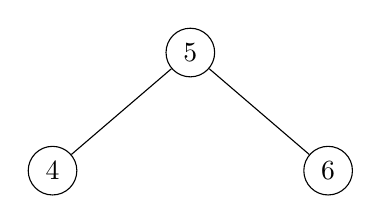
\begin{tikzpicture}
[level distance=1.5cm,
level 1/.style={sibling distance=3.5cm},
level 2/.style={sibling distance=1cm}]
\tikzstyle{every node}=[circle,draw]
\node (Root)  {5}
    child {
    node {4} } 
	child {
    node {6}
};
\end{tikzpicture}
\end{figure}



\subsection{Inserting into a binary search tree}

Inserting into a binary search tree is easy: the insert vertex just
has to obey the binary search constraint: start at the root, if the
root value is equal to the key you're inserting then go left, otherwise
go right. Once you hit a \texttt{None }create a new vertex. Running
time is $O\left(\lg n\right)$ if the tree is balanced.
\begin{algorithm}[H]
\noindent \begin{raggedright}
\texttt{Binary-Tree-Insert}$\left(B,k\right)$
\par\end{raggedright}

\begin{lstlisting}[basicstyle={\ttfamily},language=Python,mathescape=true,numbers=left,showstringspaces=false,tabsize=3]
# $B$ is a btree dict as described above, corresponding to the
# root of the tree
$prnt = ptr = B$
while $ptr \neq \text{None}$:
	# because of python's memory model we need to keep track
	# of parent since names are references not pointers, i.e.
	# you can't reassign pointers like in C
	$ prnt = ptr$
	if $ptr\left[\text{'val'}\right] \leq k$:
		$ptr = ptr\left[\text{'lchild'}\right]$
	else:
		$ptr = ptr\left[\text{'rchild'}\right]$
if $prnt\left[\text{'val'}\right] \leq k$
	$prnt\left[\text{'lchild'}\right] = \text{btree}\left(prnt,\text{next}\left(c\right),k,\text{None},\text{None}\right)$
	return $prnt\left[\text{'lchild'}\right]$
else:
	$prnt\left[\text{'rchild'}\right] = \text{btree}\left(prnt,\text{next}\left(c\right),k,\text{None},\text{None}\right)$	
	return $prnt\left[\text{'rchild'}\right]$
\end{lstlisting}
\end{algorithm}



\subsection{Searching a binary search tree}

Searching is easy because a binary search tree obey the binary search
constraint: start at the root, if the root value is equal to the key
you're searching for then you're done, otherwise if the key is less
than the value go left, otherwise go right. Running time is $O\left(\lg n\right)$
if the tree is balanced.
\begin{algorithm}[H]
\noindent \begin{raggedright}
\texttt{Binary-Tree-Search}$\left(B,k\right)$
\par\end{raggedright}

\begin{lstlisting}[basicstyle={\ttfamily},language=Python,mathescape=true,numbers=left,showstringspaces=false,tabsize=3]
$ptr = B$
while $ptr \neq \text{None}$ and $ptr\left[\text{'val'}\right] \neq k$:
	if $ptr\left[\text{'val'}\right] < k$:
		$ptr = ptr\left[\text{'lchild'}\right]$
	else:
		$ptr = ptr\left[\text{'rchild'}\right]$
if $ptr == \text{None}$:
	return "Error: key missing"
else:
	return $ptr$	
\end{lstlisting}
\end{algorithm}



\subsection{Binary search tree min/max}

The minimum of a binary tree is the left-est most vertex. Running
time is $O\left(\lg n\right)$ if the tree is balanced.

\begin{algorithm}[H]
\noindent \begin{raggedright}
\texttt{Binary-Tree-Min}$\left(B\right)$
\par\end{raggedright}

\begin{lstlisting}[basicstyle={\ttfamily},language=Python,mathescape=true,numbers=left,showstringspaces=false,tabsize=3]
$ptr = B$
while $ptr\left[\text{'lchild'}\right] \neq $None:
	$ptr = ptr\left[\text{'lchild'}\right]$
return $ptr$
\end{lstlisting}
\end{algorithm}


The maximum of a binary tree is the right-est most vertex. Running
time is $O\left(\lg n\right)$ if the tree is balanced.

\begin{algorithm}[H]
\noindent \begin{raggedright}
\texttt{Binary-Tree-Max}$\left(B\right)$
\par\end{raggedright}

\begin{lstlisting}[basicstyle={\ttfamily},language=Python,mathescape=true,numbers=left,showstringspaces=false,tabsize=3]
$ptr = B$
while $ptr\left[\text{'rchild'}\right] \neq $None:
	$ptr = ptr\left[\text{'rchild'}\right]$
return $ptr$
\end{lstlisting}
\end{algorithm}



\subsection{Binary search tree predecessor/successor}

The predecessor of a vertex the maximum of a vertex's left subtree.
Running time is $O\left(\lg n\right)$ if the tree is balanced.

\begin{algorithm}[H]
\noindent \begin{raggedright}
\texttt{Binary-Tree-Predecessor}$\left(B,k\right)$
\par\end{raggedright}

\begin{lstlisting}[basicstyle={\ttfamily},language=Python,mathescape=true,numbers=left,showstringspaces=false,tabsize=3]
$ptr = \text{Binary-Tree-Search}\left(B,k\right)$
return Binary-Tree-Max$\left(ptr\left[\text{'lchild'}\right]\right)$
\end{lstlisting}
\end{algorithm}


The successor of a vertex the minimum of a vertex's right subtree.
Running time is $O\left(\lg n\right)$ if the tree is balanced.

\begin{algorithm}[H]
\noindent \begin{raggedright}
\texttt{Binary-Tree-Predecessor}$\left(B,k\right)$
\par\end{raggedright}

\begin{lstlisting}[basicstyle={\ttfamily},language=Python,mathescape=true,numbers=left,showstringspaces=false,tabsize=3]
$ptr = \text{Binary-Tree-Search}\left(B,k\right)$
return Binary-Tree-Min$\left(ptr\left[\text{'rchild'}\right]\right)$
\end{lstlisting}
\end{algorithm}



\subsection{Deleting from a binary search tree}

We need an auxiliary function to wrap up some code that's re-used.
Running time is constant.

\begin{algorithm}[H]
\noindent \begin{raggedright}
\texttt{Transplant}$\left(u,v\right)$
\par\end{raggedright}

\begin{lstlisting}[basicstyle={\ttfamily},language=Python,mathescape=true,numbers=left,showstringspaces=false,tabsize=3]
# does not handle case where $u$ is root of tree
$prnt = u\left[\text{'parent'}\right]$
if $prnt\left[\text{'lchild'}\right] == u$
	$prnt\left[\text{'lchild'}\right] = v$
else:
	$prnt\left[\text{'rchild'}\right] = v$
if $v \neq $None:
	$v\left[\text{'parent'}\right] = prnt$
\end{lstlisting}
\end{algorithm}


Deleting from a binary search tree is a little more complicated. Since
the binary search tree property needs to be always preserved it's
unclear what to replace a deleted vertex with. A child? A parent?
In fact it should be the successor (or predecessor). The successor
is the vertex whose value would follow the vertex you're trying to
delete if you listed all the vertices in order. How do you find the
successor? It's the minimum of the right subtree or the vertex (and
the minimum of a tree is the farthest left of the tree). Then that
minimum can be replaced by it's right child (it has no left child).
Running time is $O\left(\lg n\right)$ if the tree is balanced.

\begin{algorithm}[H]
\noindent \begin{raggedright}
\texttt{Binary-Tree-Delete}$\left(B,k\right)$
\par\end{raggedright}

\begin{lstlisting}[basicstyle={\ttfamily},language=Python,mathescape=true,numbers=left,showstringspaces=false,tabsize=3]
$ptr = \text{Binary-Tree-Search}\left(B,k\right)$
# trivial case, successor is parent
if $ptr\left[\text{'rchild'}\right] == \text{None}$:
	Transplant$\left(ptr,ptr\left[\text{'lchild'}\right]\right)$
elif $ptr\left[\text{'lchild'}\right] == \text{None}$:
	Transplant$\left(ptr,ptr\left[\text{'rchild'}\right]\right)$
else:
	$succ = \text{Binary-Tree-Successor}\left(ptr\right)$
	# if the successor is the right child of $ptr$ then
	# then right child has no left child and task simple
	if $succ == ptr\left[\text{'rchild'}\right]$:
		Transplant$\left(ptr,succ\right)$
		$succ\left[\text{'lchild'}\right] = ptr\left[\text{'lchild'}\right]$
		$succ\left[\text{'lchild'}\right]\left[\text{'parent'}\right] = succ$
	else: # otherwise we have to fix successor subtrees and do the same thing 
		   # including fixing the right child
		# fix successor
		Transplant$\left(succ,succ\left[\text{'rchild'}\right]\right)$
		# don't lose right child of $ptr$
		$succ\left[\text{'rchild'}\right] = ptr\left[\text{'rchild'}\right]$
		$succ\left[\text{'rchild'}\right]\left[\text{'parent'}\right] = succ$
		# move successor into $ptr$'s position
		Transplant$\left(ptr,succ\right)$
		$succ\left[\text{'lchild'}\right] = ptr\left[\text{'lchild'}\right]$
		$succ\left[\text{'lchild'}\right]\left[\text{'parent'}\right] = succ$		
\end{lstlisting}
\end{algorithm}



\subsection{Pre-order/In-order/Post-order traversal}

A Pre-order/In-order/Post-order traversal of a binary tree is a traversal
the manipulates the vertex either before left and right children,
after the left child but before the right child, and after both the
left and right children. The easiest way to implement any of these
is recursion but iterative versions do exist. Running time is $O\left(n\right)$
since the traversal visits every vertex. For illustrative purposes
we simply print the \texttt{val }attribute, but any operation on the
vertex could be performed.

\begin{algorithm}[H]
\noindent \begin{raggedright}
\texttt{Pre-order-traversal}$\left(B\right)$
\par\end{raggedright}

\begin{lstlisting}[basicstyle={\ttfamily},language=Python,mathescape=true,numbers=left,showstringspaces=false,tabsize=3]
print$\left(B\left[\text{'val'}\right]\right)$
Pre-order-traversal$\left(B\left[\text{'lchild'}\right]\right)$
Pre-order-traversal$\left(B\left[\text{'rchild'}\right]\right)$
\end{lstlisting}
\end{algorithm}
\begin{algorithm}[H]
\noindent \begin{raggedright}
\texttt{In-order-traversal}$\left(B\right)$
\par\end{raggedright}

\begin{lstlisting}[basicstyle={\ttfamily},language=Python,mathescape=true,numbers=left,showstringspaces=false,tabsize=3]
Pre-order-traversal$\left(B\left[\text{'lchild'}\right]\right)$
print$\left(B\left[\text{'val'}\right]\right)$
Pre-order-traversal$\left(B\left[\text{'rchild'}\right]\right)$
\end{lstlisting}
\end{algorithm}
\begin{algorithm}[H]
\noindent \begin{raggedright}
\texttt{Post-order-traversal}$\left(B\right)$
\par\end{raggedright}

\begin{lstlisting}[basicstyle={\ttfamily},language=Python,mathescape=true,numbers=left,showstringspaces=false,tabsize=3]
Pre-order-traversal$\left(B\left[\text{'lchild'}\right]\right)$
Pre-order-traversal$\left(B\left[\text{'rchild'}\right]\right)$
print$\left(B\left[\text{'val'}\right]\right)$ 
\end{lstlisting}
\end{algorithm}



\section{Treap}

Binary trees have $O\left(\lg n\right)$ queries and inserts and deletions
if they're balanced. Turns out keep them balanced is tough - a ton
of schemes exist. The simpliest is a random binary tree using a treap.
A treap combines the invariants of a binary tree \emph{and} and a
heap. There are two sets of attributes: priorities and keys. The priorities
obey the heap property (children have smaller priority than their
parents) and the keys obey the binary search property. In order to
get a balanced binary tree, which is the value of treaps, we randomly
generate a priority key. This then simulates the generation of a random
binary tree which on average has depth $O\left(\lg n\right)$. We
use a min heap.


\subsection{Treap search}

Just like for binary search tree and hence omitted.


\subsection{Treap insert}

This is easier of the two operations. First we need two auxiliary
functions \texttt{Left-Rotate} and \texttt{Right-Rotate}. The easiest
way to remember these is pictures

\begin{figure}[H]


\noindent \begin{centering}
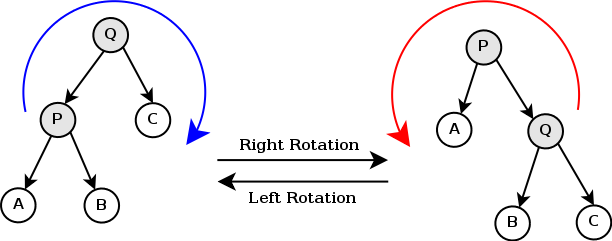
\includegraphics[scale=0.5]{Tree_rotation}
\par\end{centering}

\end{figure}
\begin{algorithm}[H]
\noindent \begin{raggedright}
\texttt{Left-rotate}$\left(p\right)$
\par\end{raggedright}

\begin{lstlisting}[basicstyle={\ttfamily},language=Python,mathescape=true,numbers=left,showstringspaces=false,tabsize=3]
$p_{prnt} = p\left[\text{'parent'}\right]$
$a = p\left[\text{'lchild'}\right]$
$q = p\left[\text{'rchild'}\right]$
# put $q$ in $p$'s position
if $p = p_{prnt}\left[\text{'lchild'}\right]$:
	$p_{prnt}\left[\text{'lchild'}\right] = q$
else:
	$p_{prnt}\left[\text{'rchild'}\right] = q$
$p\left[\text{'rchild'}\right] = q\left[\text{'lchild'}\right]$
$q\left[\text{'lchild'}\right] = p$
\end{lstlisting}
\end{algorithm}
\begin{algorithm}[H]
\noindent \begin{raggedright}
\texttt{Right-rotate}$\left(p\right)$
\par\end{raggedright}

\begin{lstlisting}[basicstyle={\ttfamily},language=Python,mathescape=true,numbers=left,showstringspaces=false,tabsize=3]
$q_{prnt} = q\left[\text{'parent'}\right]$
$p = q\left[\text{'lchild'}\right]$
$c = q\left[\text{'rchild'}\right]$
# put $p$ in $q$'s position
if $q = q_{prnt}\left[\text{'lchild'}\right]$:
	$q_{prnt}\left[\text{'lchild'}\right] = p$
else:
	$q_{prnt}\left[\text{'rchild'}\right] = p$
$q\left[\text{'lchild'}\right] = p\left[\text{'rchild'}\right]$
$p\left[\text{'rchild'}\right] = q$
\end{lstlisting}
\end{algorithm}


To insert into a treap, generate a random priority, and insert the
key as if it were a binary search tree (i.e. at the bottom), then
rotate up until the heap property is restored.

\begin{algorithm}[H]
\noindent \begin{raggedright}
\texttt{Treap-Insert}$\left(T,k\right)$
\par\end{raggedright}

\begin{lstlisting}[basicstyle={\ttfamily},language=Python,mathescape=true,numbers=left,showstringspaces=false,tabsize=3]
# $T$ is a binary tree that's a treap
$u = \text{Random}\left(0,1\right)$ # both ends inclusive
$ptr = \text{Binary-Tree-Insert}\left(T,\left(u,k\right)\right)$
$prnt = ptr\left[\text{'parent'}\right]$
while $prnt \neq \text{None}$ and $ptr\left[\text{'val'}\right] < prnt\left[\text{'val'}\right]$:
	if $ptr == prnt\left[\text{'lchild}\right]$:
		Right-Rotate$\left(prnt\right)$
	else:
		Left-Rotate$\left(prnt\right)$
	$ptr = prnt$
	$prnt = ptr\left[\text{'parent'}\right]$	
\end{lstlisting}
\end{algorithm}



\subsection{Treap delete}

To delete a vertex rotate it down until it's a leaf node and then
delete the leaf node. Rotate down according to which of the vertex's
children have a higher priority: if the left child has a higher priority
than the right then rotate right, otherwise rotate left.
\begin{algorithm}[H]
\noindent \begin{raggedright}
\texttt{Treap-Delete}$\left(T,k\right)$
\par\end{raggedright}

\begin{lstlisting}[basicstyle={\ttfamily},language=Python,mathescape=true,numbers=left,showstringspaces=false,tabsize=3]
# $T$ is a binary tree that's a treap

$ptr = \text{Binary-Tree-Search}\left(T,k\right)$
while $ptr\left[\text{'lchild'}\right] \neq \text{None}$ or $ptr\left[\text{'lchild'}\right] \neq \text{None}$:
	if $ptr\left[\text{'lchild'}\right] \neq \text{None}$ and $ptr\left[\text{'lchild'}\right]\left[\text{'val'}\right] > ptr\left[\text{'rchild'}\right]\left[\text{'val'}\right]$
		Right-Rotate$\left(ptr\right)$
	else:
		Left-Rotate$\left(ptr\right)$
	if $ptr = ptr\left[\text{'parent'}\right]\left[\text{'lchild'}\right]$:
		$ptr\left[\text{'parent'}\right]\left[\text{'lchild'}\right] = \text{None}$
	else:
		$ptr\left[\text{'parent'}\right]\left[\text{'rchild'}\right] = \text{None}$
	del $ptr$
\end{lstlisting}
\end{algorithm}



\section{Cartesian Tree}

Given a sequence of \textbf{distinct} numbers (or any totally ordered
objects), there exists a binary min-heap whose inorder traversal is
that sequence. This is known as the Cartesian tree for that sequence.
A min-treap is an easy way to construct a Cartiesian tree of a sorted
sequence. Why? Obviously: it's is heap ordered since it obeys the
min heap property and an in order traversal reproduces the sequence
in sorted order. How to construct a Cartesian tree for an arbitrary
sequence $A=\left[a_{1},\dots,a_{n}\right]$? Process the sequence
values in left-to-right order, maintaining the Cartesian tree of the
nodes processed so far, in a structure that allows both upwards and
downwards traversal of the tree. To process each new value $x$, start
at the node representing the value prior to $x$ in the sequence and
follow the path from this node to the root of the tree until finding
a value $y$ smaller than $x$. This node $y$ is the parent of $x$,
and the previous right child of $y$ becomes the new left child of
$x$. Running time is $O\left(n\right)$.

\begin{algorithm}[H]
\noindent \begin{raggedright}
\texttt{Cartesian-Tree}$\left(A\right)$
\par\end{raggedright}

\begin{lstlisting}[basicstyle={\ttfamily},language=Python,mathescape=true,numbers=left,showstringspaces=false,tabsize=3]
$T = \text{btree}\left(\text{None},\text{next}\left(c\right),A\left[1\right],\text{None},\text{None}\right)$
$ptr = prnt = T$
for $i= 2:\text{len}\left(A\right)$:
	while $prnt\left[\text{'parent'}\right] \neq \text{None}$ and $A\left[i\right] <prnt\left[\text{'val}\right] $
		$prnt = prnt\left[\text{'parent'}\right]$
	if $prnt == \text{None}$: # then we're at the root
		# and $A\left[i\right]$ is the smallest value we've seen so far
		$ptr = \text{btree}\left(\text{None},\text{next}\left(c\right),A\left[i\right],prnt,\text{None}\right)$
		$prnt\left[\text{'parent'}\right] = ptr$
	else:
		$ptr = \text{btree}\left(prnt,\text{next}\left(c\right),A\left[i\right],prnt\left[\text{'rchild'}\right],\text{None}\right)$
		$prnt\left[\text{'rchild'}\right] = ptr$
	$prnt = ptr$
		
\end{lstlisting}
\end{algorithm}



\section{Interval Trees}

An interval tree is built atop your favotire balanced binary tree
data structure (treap in our case) and stores left endpoints as key.
It also keeps track of maximum right endpoint in the subtree rooted
at a vertex. It supports interval intersection tests (very useful).
Maintaining the max in insertion and deletion is straightforward during
rotations.


\subsection{Interval search}

Interval search works by being optimistic: $i=\left[a,b\right]$ and
$j=\left[x,y\right]$ two intervals overlap if either $a\leq x\leq b$
or $x\leq a\leq y$. Therefore at each interval we test for overlap
and whether $x\leq a\leq y$ where $y$ is the maximum right endpoint
for any interval in the left subtree. If so we go left. If in fact
$y<a$ then no interval in the left subtree could possibly intersect
so we go right.

\begin{algorithm}[H]
\noindent \begin{raggedright}
\texttt{Interval-Tree-Search}$\left(T,i\right)$
\par\end{raggedright}

\begin{lstlisting}[basicstyle={\ttfamily},language=Python,mathescape=true,numbers=left,showstringspaces=false,tabsize=3]
# $T$ is an interval tree, $i = \left[a,b\right]$
$a,b = i\left[1\right],i\left[2\right]$
# $j\left[\text{'left'}\right]$ is left endpoint of interval and 
# $j\left[\text{'right'}\right]$ is right endpoint
intersect $=$ lamba $j$: $a \leq j\left[\text{'left'}\right] \leq b$ or $j\left[\text{'left'}\right] \leq a \leq j\left[\text{'right'}\right]$
# 'int' is interval associated with vertex
while $T \neq \text{None}$ and not intersect$\left(T\left[\text{'int'}\right]\right)$:
	if $T\left[\text{'lchild'}\right] \neq \text{None}$ and $a \leq T\left[\text{'lchild'}\right]\left[\text{'max'}\right]$:
		$T = T\left[\text{'lchild'}\right]$
	else:
		$T = T\left[\text{'rchild'}\right]$
return $T$
\end{lstlisting}
\end{algorithm}



\section{Order Statistics Tree}

Order statistics trees are probably the simplest thing to build atop
a balanced binary search tree. The only extra extra piece of information
each vertex stores is the attribute \texttt{size }where $x\left[\texttt{'size'}\right]=x\left[\texttt{'lchild'}\right]\left[\texttt{'size'}\right]+x\left[\texttt{'rchild'}\right]\left[\texttt{'size'}\right]+1$.


\subsection{Select}

Finding the $i$th ordered element in the tree works just like Quickselect

\begin{algorithm}[H]
\noindent \begin{raggedright}
\texttt{OS-Select}$\left(T,i\right)$
\par\end{raggedright}

\begin{lstlisting}[basicstyle={\ttfamily},language=Python,mathescape=true,numbers=left,showstringspaces=false,tabsize=3]
# $T$ is an interval tree, $i$ is the rank we're looking for
$r = T\left[\text{'lchild'}\right]\left[\text{'size'}\right] + 1 $
if $i == r$:
	return $x$
elif $i < r$:
	return OS-Select$\left(T\left[\text{'lchild'}\right],i\right)$
else:
	return OS-Select$\left(T\left[\text{'rchild'}\right],i-r\right)$
\end{lstlisting}
\end{algorithm}



\subsection{Rank}

We can find the rank of an element by finding how many elements are
to its left.

\begin{algorithm}[H]
\noindent \begin{raggedright}
\texttt{OS-Rank}$\left(T,x\right)$
\par\end{raggedright}

\begin{lstlisting}[basicstyle={\ttfamily},language=Python,mathescape=true,numbers=left,showstringspaces=false,tabsize=3]
$x$ is a pointer to a vertex in the tree
$r  = x\left[\text{'lchild'}\right]\left[\text{'size'}\right] + 1 $
$prnt = x$
# while $prnt$ is not root of $T$
while $prnt \neq T$:
	if $ prnt == prnt\left[\text{'parent'}\right]\left[\text{'rchild'}\right]$:
		$r  = r+ prnt\left[\text{'parent'}\right]\left[\text{'lchild'}\right]\left[\text{'size'}\right] + 1 $
	$prnt = prnt\left[\text{'parent'}\right]$
return $r$
\end{lstlisting}
\end{algorithm}



\subsection{Maintenance}

Maintaining \texttt{size }is easy: for example in \texttt{Left-Rotate
}add lines \\
\\
13 $y\left[\texttt{'size'}\right]=x\left[\texttt{'size'}\right]$\\
14 $x\left[\texttt{'size'}\right]=x\left[\texttt{'lchild'}\right]\left[\texttt{'size'}\right]+x\left[\texttt{'rchild'}\right]\left[\texttt{'size'}\right]+1$

and similarly for \texttt{Right-Rotate.}


\section{Union-Find}

A union-find data structure is a data structure suited for taking
unions and finding members (duh). The particular units of the data
structures are sets (not hash table derivatives), each with a representative.
The data structure is very thin, basically a wrapper for the primitive
data, except for a pointer to the representative of the set and two
heuristics that speed up the operations. The path compression heuristic
``compresses'' the path to representative of the set by setting
it to be equal to that representative (which it might not be after
a union). The weighted union heuristic makes it so that the smaller
of the two sets unioned is the one whose representative pointers need
to be updated.

Amortized complexity of $n$ \texttt{Make-Set}, \texttt{Find-Set,
Union,} operations where $m$ are \texttt{Make-Set} is $O\left(m\alpha\left(n\right)\right)$
where $\alpha\left(n\right)$ is the Ackermann function and $\alpha\left(n\right)\leq4$
for any realistic application.


\subsection{Make set}

\begin{algorithm}[H]
\noindent \begin{raggedright}
\texttt{Make-Set}$\left(x\right)$
\par\end{raggedright}

\begin{lstlisting}[basicstyle={\ttfamily},language=Python,mathescape=true,numbers=left,showstringspaces=false,tabsize=3]
return {'val':$x$,'rep':$x$,'rank':0}
\end{lstlisting}
\end{algorithm}



\subsection{Find set}

Find set is interesting: it unwinds the stack in order to reset all
the representatives from $x$ to the representative of the set.

\begin{algorithm}[H]
\noindent \begin{raggedright}
\texttt{Find-Set}$\left(x\right)$
\par\end{raggedright}

\begin{lstlisting}[basicstyle={\ttfamily},language=Python,mathescape=true,numbers=left,showstringspaces=false,tabsize=3]
if $x\left[\text{'rep'}\right]\neq x$:
	$x\left[\text{'rep'}\right] = \text{Find-Set}\left(x\left[\text{'rep'}\right]\right)$
\end{lstlisting}
\end{algorithm}



\subsection{Union}

Find set is interesting: it unwinds the stack in order to reset all
the representatives from $x$ to the representative of the set. Running
time is $O\left(m\lg n\right)$.

\begin{algorithm}[H]
\noindent \begin{raggedright}
\texttt{Union}$\left(x,y\right)$
\par\end{raggedright}

\begin{lstlisting}[basicstyle={\ttfamily},language=Python,mathescape=true,numbers=left,showstringspaces=false,tabsize=3]
$x_{rep} = \text{Find-Set}\left(x\right)$
$y_{rep} = \text{Find-Set}\left(y\right)$
if $x_{rep}\left[\text{'rank'}\right] > y_{rep}\left[\text{'rank'}\right]$
	$y_{rep}\left[\text{'rep'}\right] = x_{rep}$
else:
	$x_{rep}\left[\text{'rep'}\right] = y_{rep}$
	if $x_{rep}\left[\text{'rank'}\right] == y_{rep}\left[\text{'rank'}\right] $
		# it's an approximate rank.
		$y_{rep}\left[\text{'rank'}\right] = y_{rep}\left[\text{'rank'}\right] + 1$
\end{lstlisting}
\end{algorithm}



\section{Euler circuit}

An Euler circuit visits each vertex in graph twice - once going past
it and once coming back across it. How do you print out an Euler circuit
of a tree? Use a modified depth first traversal.
\begin{algorithm}[H]
\noindent \begin{raggedright}
\texttt{Euler-Circuit}$\left(u\right)$
\par\end{raggedright}

\begin{lstlisting}[basicstyle={\ttfamily},language=Python,mathescape=true,numbers=left,showstringspaces=false,tabsize=3]
# $u$ is a vertex with children
# print it going past
print$\left(u\right)$
for $v$ in $u\left[\text{'children'}\right]$:
	Euler-Circuit$\left(v\right)$
	# print is coming back
	print$\left(u\right)$
\end{lstlisting}
\end{algorithm}



\section{Tarjan's Least Common Ancestor}

The least common ancestor $w$ of two vertices $u,v$ in a tree is
the ancestor common to both that's of greatest depth. The algorithm
is useful for range-minimum querying. It uses the same traversal as
\texttt{Euler-Circuit} and the Union-Find data structure augmented
with a property \texttt{ancestor}. The algorithm proceeds by growing
``bottom up'' sets corresponding to subtrees whose roots are the
least common ancestors of any pair of vertices in the tree \textbf{which
have been completely traversed by the Euler circuit}. Let $P$ be
a global with the set of vertices you're interested in finding least
common ancestor of and initialize all vertices to have \texttt{color
}\textcolor{blue}{Blue} in order to represent unfinishined (i.e. not
completely traversed by the Euler circuit).

\begin{algorithm}[H]
\noindent \begin{raggedright}
\texttt{Least-Common-Ancestor}$\left(u\right)$
\par\end{raggedright}

\begin{lstlisting}[basicstyle={\ttfamily},language=Python,mathescape=true,numbers=left,showstringspaces=false,tabsize=3]
# $u$ is the root of a tree
$u_{set} = \text{Make-Set}\left(u\right)$
#this is the Euler-Circuit transformation (equivalent of print)
$u_{set}\left[\text{'ancestor'}\right]= u$
for $v$ in $u\left[\text{'children'}\right]$:
	$\text{Least-Common-Ancestor}\left(v\right)$
	# let's pretend there's a big table where i can fetch $v_{set}$ from
	Union$\left(u_{set},v_{set}\right)$
	$u_{set}\left[\text{'ancestor'}\right]= u$
# $u_{set}\left[\text{'val'}\right] = u$
$u_{set}\left[\text{'val'}\right]\left[\text{'color'}\right] = \color{red}\text{Red}$
for each $v$ such that $\{u,v\} \in P$:
	if $v\left[\text{'color'}\right] == \color{red}\text{Red}$:
		print$\left(\text{"Least common ancestor of } \{u,v\} \text{ is " } + v_{set}\left[\text{'ancestor'}\right]\right)$
\end{lstlisting}
\end{algorithm}



\section{Range Minimum Queries}

Given a sequence of distinct values and a subsequence (specified by
it's end points) what is the minimum value of the in that subsequences?
It's just the least common ancestor of the end points in the cartesian
tree representing the sequence.


\part{Advanced Design Techniques}


\section{Dynamic Programming}

Note this is a fairly formal explanation of dynamic programming. Skip
if you're not interested in formalism. If you want a good intuitive
interpretation of Dynamic programming read chapter 6 of Vazirani (where
he says that dynamic programming is simply traversing the topological
sort of the problem dependency graph).

Dynamic programming does not means writing code dynamically or changing
code dynamically or anything like that. The sense in which programming
is being used here is the same sense as setting a program for an festival
or something, and dynamic means making decisions in-situ rather than
a priori. dynamic programming is an optimization technique - minimizing
travel time, minimizing cost, maximizing profits, maximizing utility,
et cetera. The central concept is the \textbf{Bellman equation} so
I'm going to crib here the wikipedia article on the Bellman equation
(yes the whole thing). 

First, any optimization problem has some objective \textendash{} minimizing
travel time, minimizing cost, maximizing profits, maximizing utility,
et cetera. The function that describes this objective is called the
\textbf{objective function} or \textbf{cost function},i.e. the travel
time, cost, or profits as a function of time. Dynamic programming
breaks a multi-period planning problem into simpler steps. Therefore,
it requires keeping track of how the circumstances, as the concern
the decision at each step, change over time. The information about
the current situation which is needed to make a correct decision is
called the ``state\textquotedbl{}. For example, to decide how much
to consume and spend at each point in time, people would need to know
(among other things) their initial wealth. Therefore, current wealth
would be one of their \textbf{state variables}. The decisions made
at each step are represented by \textbf{control variables}.\textbf{
}For example, in the simplest case, today's wealth (the state) and
how much is consumed (the control) determine tomorrow's wealth (the
new state).

The dynamic programming approach describes the optimal plan by finding
a rule that tells what the controls should be, given any possible
value of the state. For example, if consumption $c$ depends only
on wealth $W$, we would seek a rule $c\left(W\right)$ that gives
consumption as a function of wealth. Such a rule, determining the
controls as a function of the states, is called a \textbf{policy function}.

Finally, by definition, the optimal decision rule is the one that
achieves the best possible value of the objective. For example, if
someone chooses consumption, given wealth (wealth is fixed), in order
to maximize happiness (assuming happiness $H$ can be represented
by a function, such as a \textbf{utility function}), then each level
of wealth will be associated with some highest possible level of happiness,
$H\left(W\right)$. The best possible value of the objective, written
as a function of the state, is called the \textbf{value function}.

I have no idea what this value function is and how it is distinct
from the objective function (but I guess I'll find out).

Richard Bellman showed that a dynamic optimization problem in discrete
time can be stated in a recursive, step-by-step form known as \textbf{backward
induction} by writing down the relationship between the value function\footnote{This has gotta mean cost function,or imply that the value function
is the cost function.} in one period and the value function in the next period. The relationship
between these two value functions is called the \textquotedbl{}Bellman
equation\textquotedbl{}. In this approach, the optimal policy in the
final time period is specified in advance as a function of the state
variable's value at that time, and the resulting optimal value of
the objective function is thus expressed in terms of that value of
the state variable. Next, the next-to-final period's optimization
involves maximizing the sum of that period's period-specific objective
function and the optimal value of the future objective function, giving
that period's optimal policy contingent upon the value of the state
variable as of the next-to-last period decision. This logic continues
recursively back in time, until the first period decision rule is
derived, as a function of the initial state variable value, by optimizing
the sum of the first-period-specific objective function and the value
of the second period's value function, which gives the value for all
the future periods. Thus, each period's decision is made by explicitly
acknowledging that all future decisions will be optimally made.


\subsection{Fibonacci Sequence}

The simplest dynamic programming algorithm is computing the $n$th
Fibonacci number faster than using the naive recursive definition
\[
F_{n}=F_{n-1}+F_{n-2}
\]
What's the idea? Overlapping substructure: look at the ``call stack''
for trying to compute $F_{n}$

\begin{figure}[H]
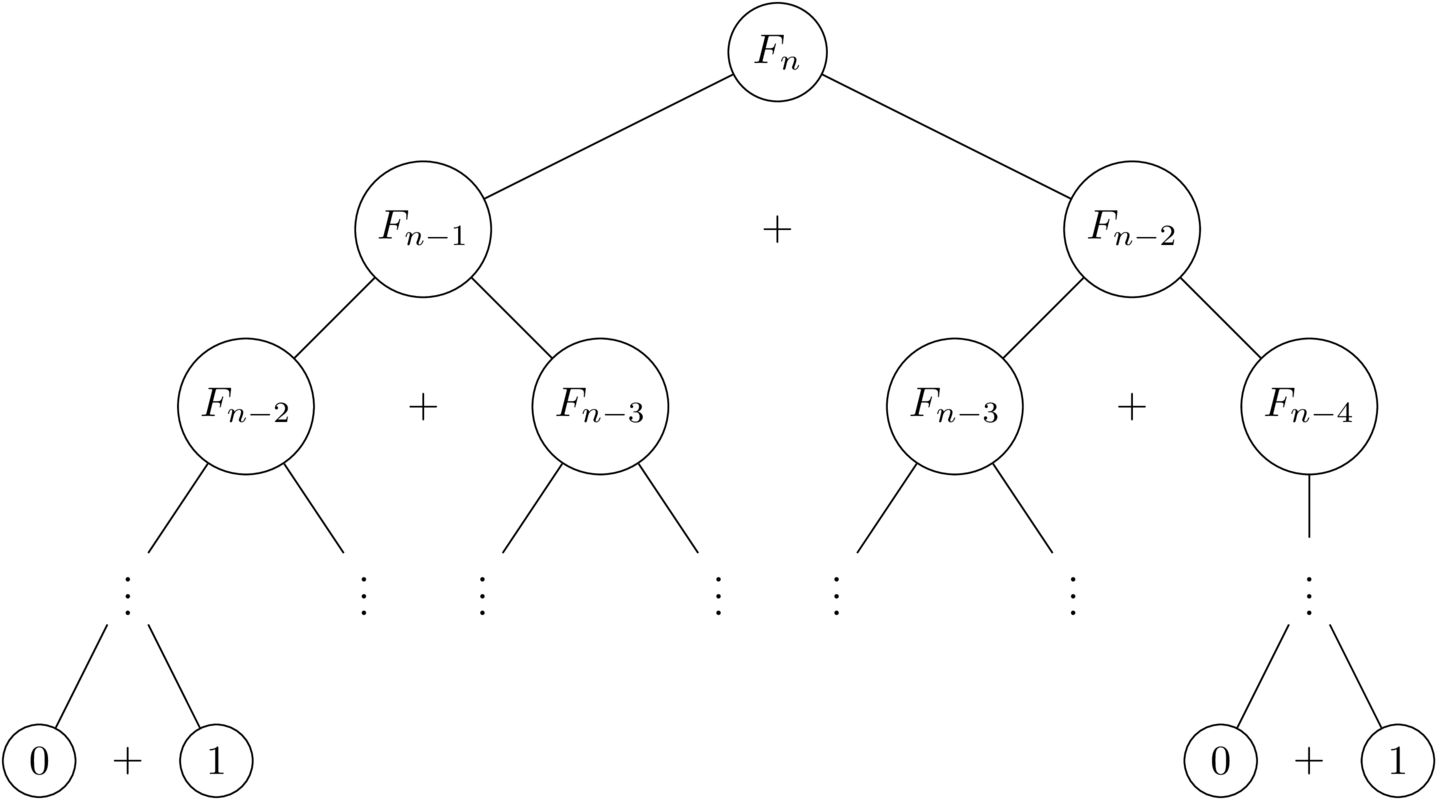
\includegraphics[scale=0.25]{fib}
\end{figure}


Look at all of the repeated calls to $F_{j}$. Rewrite the calculation
so that there's no redundant work. There are two ways to do this:
using a hashtable to memoize calls or do the computation bottom up.
Running time is $O\left(n\right)$.

\begin{algorithm}[H]
\noindent \begin{raggedright}
\texttt{Fibonacci}$\left(n\right)$
\par\end{raggedright}

\begin{lstlisting}[basicstyle={\ttfamily},language=Python,mathescape=true,numbers=left,showstringspaces=false,tabsize=3]
if $n == 1$ or $n == 2$:
	return $1$
else:
	$F_{k-1} = 1$
	$F_{k} = 1$
	$k = 2$
	while $k < n$:
		# k is not a parameter, subscripts are labels not indices
		$F_{k+1} = F_k + F_{k-1}$
		$F_k = F_{k+1}$
		$F_{k-1} = F_k$
		$k = k+1$ 
return $F_{k+1}$
\end{lstlisting}
\end{algorithm}



\subsection{Rod Cutting}

Given a rod of length $n$ and a table of price $P=\left[p_{1},\dots,p_{n}\right]$
corresponding to cuts at $i$ units of length what's the maximum value
$r_{n}$ obtained by cutting up the rod? The naive solution is to
try all $2^{n-1}$ partitions of the rod. Clearly not efficient. The
optimal substructure of the problem is such the maximum value is the
sum of maximum value of the potential partitions around a particular
cut, and not cutting at all. Therefore the Bellman equation is
\[
r_{i}=\max\left\{ p_{i},r_{1}+r_{i-1},r_{1}+r_{i-1},r_{2}+r_{i-2},\dots,r_{i-1}+r_{1}\right\} =\max_{j=1,\dots,i}\left\{ p_{i},r_{j}+r_{i-j}\right\} 
\]
Notice the duplication in the first expression, which corresponds
to mirror symmetry of the rod (turning the rod around maps a cut $r_{j}+r_{i-j}$
to $r_{i-j}+r_{j}$). Therefore the less redundant Bellman equation
is 
\[
r_{i}=\max_{j<i-j}\left\{ p_{i},r_{j}+r_{i-j}\right\} 
\]
An equivalent formulation (all cuts of this form correspond to all
cuts of the prior form) is one solid piece of length $i$ and a potentially
further subdivided piece of length $n-i$. Therefore the Bellman equation
is (with the $r_{0}\equiv0$) 
\[
r_{i}=\max_{j=1,\dots,i}\left\{ p_{j}+r_{i-j}\right\} 
\]
The naive recursive implementation runs in $O\left(2^{n}\right)$
because it recomputes solutions to subproblems several times unnecessarily.

\begin{algorithm}[H]
\noindent \begin{raggedright}
\texttt{Rod-Cut-Rec}$\left(P,n\right)$ 
\par\end{raggedright}

\begin{lstlisting}[basicstyle={\ttfamily},language=Python,mathescape=true,numbers=left,showstringspaces=false,tabsize=3]
if $n == 0$:
	return $0$
$r = -\infty$
for $i = 1:n$:
	$r=\max\left\{ r,P\left[i\right]+\text{Rod-Cut-Rec}\left(P,n-i\right)\right\} $
return $r$
\end{lstlisting}
\end{algorithm}


To speed this up you need to ``memoize'' redundant calls (hash table
with already computed values) \emph{or} compute values bottom up.
The more elegant solution solution is the bottom up computation.

\begin{algorithm}[H]
\noindent \begin{raggedright}
\texttt{Bottom-Up-Rod-Cut}$\left(P,n\right)$ 
\par\end{raggedright}

\begin{lstlisting}[basicstyle={\ttfamily},language=Python,mathescape=true,numbers=left,showstringspaces=false,tabsize=3]
$ r = n\cdot \left[0\right]$
for $i = 1:n$:
	$q = 0$
	for $j=1:i$:
		# recall $r\left[0\right] \equiv 0$
		$q=\max\left\{ q,P\left[i\right]+r\left[i-j\right]\right\} $
	$r\left[i\right] = q$
return $r\left[n\right]$
\end{lstlisting}
\end{algorithm}



\subsection{Getting to work\protect\footnote{This example is Applied Mathematical Programming by Bradley,Hax, Magnanti
chapter 11. }}

Given a neighborhood of $n$ commuters and $n$ downtown parking lots
what is the fastest way for each commuter to get to work given that
intersection have delays?

\begin{figure}[H]
\noindent \centering{}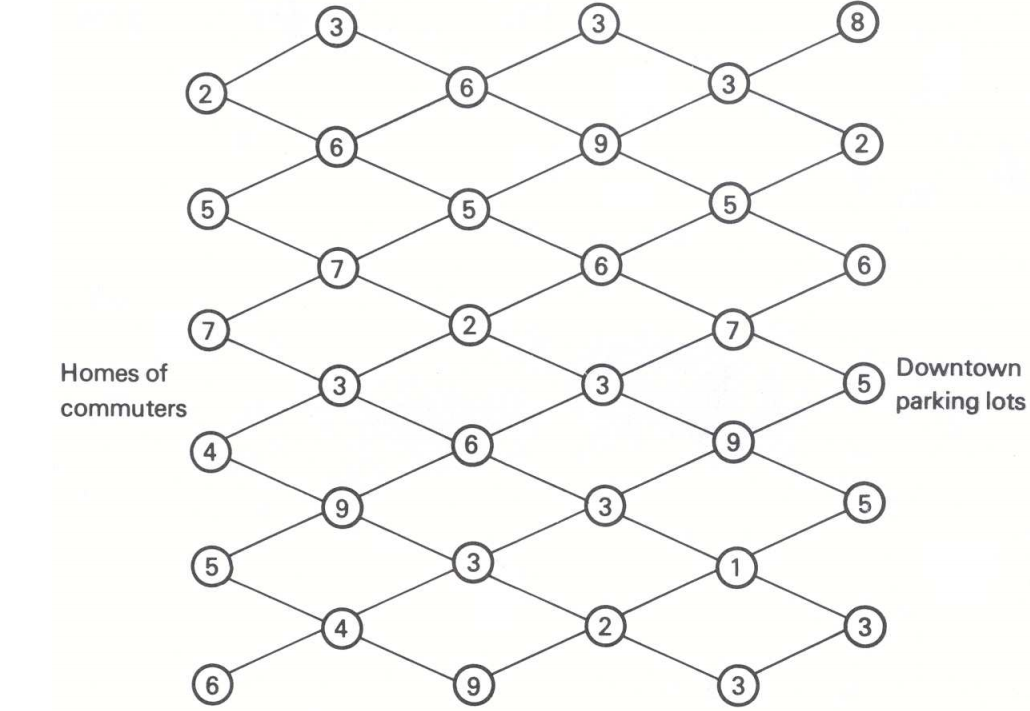
\includegraphics[scale=0.25]{commute}
\end{figure}


Imagine instersections are on a rectified grid and that the cost (in
time) of getting to intersection $i,j$ from some house is $q\left(i,j\right)$
and $c\left(i,j\right)$ is the time to get between intersection (left
to right - one way streets). Seems like you'd have to start at the
end (parking lots) and work backwards right? But no in fact this problem
has optimal substructure
\[
q\left(i,j\right)=\begin{cases}
\infty & j<1\text{ or }j>n\\
c\left(i,j\right) & i=1\\
\min\left\{ q\left(i-1,j-1\right),q\left(i-1,j+1\right)\right\} +c\left(i,j\right) & \text{otherwise}
\end{cases}
\]
Starting from any particular household $\left(1,j\right)$ we can
compute the shortest path cost to any parking lot by forward iteration.
Running time is $O\left(nk\right)$.

\begin{algorithm}[H]
\noindent \begin{raggedright}
\texttt{Shortest-Path-Parkin}g$\left(A,c\right)$
\par\end{raggedright}

\begin{lstlisting}[basicstyle={\ttfamily},language=Python,mathescape=true,numbers=left,showstringspaces=false,tabsize=3]
# $A$ is an $n\times k$ grid (or something like that)
# and $c$ is the associated costs with getting
# to the intersection
$ n = \text{len}\left(A\right)$
$q = n\cdot\left[n\cdot\left[\infty\right]\right]$
for $i=1:n$:
	# initialize first hop intersections
	$q\left[1,i\right] = c\left[1,i\right]$
for $i=2:n$:
	for $j=1:n$:
		# i'll let you figure out how to 
		# bumper the $q$ array so that 
		# when $i,j=1$ the entries
		# $q\left[i-1,j-1\right] = \infty$
		$q\left[i,j\right] = \min\left\{ q\left[i-1,j-1\right],q\left[i-1,j+1\right] \right\} +c\left[i,j\right] $
return $q$
\end{lstlisting}
\end{algorithm}
In order to return the actual path to any parking garage just modify
the \texttt{for} loop to keep track of which of $q\left(i-1,j-1\right)$
or $q\left(i-1,j+1\right)$ was chosen in the min.


\subsection{Towers of Hanoi}

Move all the disks from the left rod to the far right one only one
disk (top disk) at a time.

\begin{figure}[H]
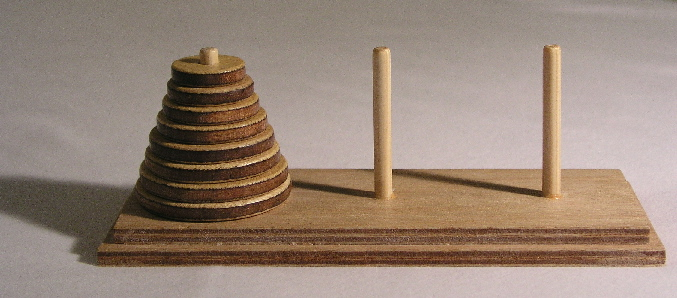
\includegraphics[scale=0.5]{Tower_of_Hanoi.jpeg}
\end{figure}


This problem has optimal substructure in that there's no real difference
between any of the rods or disks: so moving $n$ disks from the first
rod to the third involves moving $n-1$ disks (from some rod) to the
third rod. The solution is purely recursive: let $S\left(n,h,t\right)$
be the solution to moving $n$ disks from their ``home'' rod $h$
to a target rod $t$. Then 
\[
S\left(1,h,t\right)=\text{just move the disk}
\]
and 
\begin{eqnarray*}
S\left(n,h,t\right) & = & \text{first }S\left(n-1,h,\text{not}\left(h,t\right)\right)\\
 &  & \text{second }S\left(1,h,t\right)\\
 &  & \text{third }S\left(n-1,\text{not}\left(h,t\right),t\right)
\end{eqnarray*}


Running time is $O\left(2^{n}\right)$.


\subsection{Egg drop}


\subsubsection{\textbf{2 eggs 100 floors}}

Suppose you have 2 eggs and a 100 story building and we want to find
out the highest floor \emph{an} can be dropped from safely. The assumptions
are 
\begin{itemize}
\item An egg that survives a fall can be used again.
\item A broken egg must be discarded.
\item The effect of a fall is the same for all eggs.
\item If an egg breaks when dropped from some floor, then it will break
if dropped from higher floors.
\item If an egg survives a fall, then it would survive a fall from a lower
floor.
\end{itemize}
Starting from the 14th floor is the best strategy because the number
of attempts (in the worst case) is always 14. Why? If the first egg
breaks at the 14th floor then you have to check floors 1 through 13
with the second egg for a total of 14 floors. If the egg doesn't break
then move to the 27th floor. If it breaks then you have to check floors
15 through 26 for a total of $13+1=14$. Then move to the 39th floor
and etc. The sequence of floors is $14,27,39,50,60,69,77,84,90,95,99,100$.
If the egg breaks at any point before getting to floor 100 you have
to test 13 more floors. If it doesn't break until the 100th floor
then you have to perform only 12 drops.


\subsubsection{\textbf{2 eggs $k$ floors}}

Suppose that for the best strategy, the number of drops in the worst
case is $x$. Then, you should start at the $x$th floor. If the first
egg breaks then you have $x-1$ floors to check for a total of $1+\left(x-1\right)=x$
floors to check. If it doesn't break then you should check $x+\left(x-1\right)$th
floor. If it breaks then with the second egg you have to check floors
$x+1,x+2,\dots,\left(x+\left(x-1\right)-1\right)$, for a total of
\[
\left(x+\left(x-1\right)-1\right)-\left(x+1\right)+1=x-2
\]
plus the drop at floor $x$ and floor $x+\left(x-1\right)$ makes
for a total of $x$ drops.

What's actually happening is assuming that using the best strategy
the minimum number of drops is $x$ we are searching for the best
strategy that covers all of the floors. Suppose the minimum number
of attempts, in the worst case, while using the best strategy is $x$.
How many floors can we cover?

\[
x+\left(x-1\right)+\left(x-2\right)+\cdots+2+1=\frac{x\left(x+1\right)}{2}
\]
So we need 
\[
\frac{x\left(x+1\right)}{2}\geq k
\]
or 
\[
x=\left\lceil \frac{-1+\sqrt{1+8k}}{2}\right\rceil 
\]
which for $k=100$ implies $x=14$.


\subsubsection{\textbf{N eggs, k floors}}

Suppose you have $n$ eggs, $h$ consecutive floors to be tested,
and you drop an egg at floor $i$ in this sequence of $h$ floors.
If the egg breaks then the problem reduces to $n-1$ eggs and $i-1$
remaining floors. If the egg doesn't break then the problem reduces
to $n$ eggs and $h-i$ remaining floors. This is the optimal substructure
of the problem: the floors we want to test are irrelevant, only their
quantity. Let $W\left(n,h\right)$ be the minimum number of drops
required to find the threshold floor in the worst case, while using
the best strategy. Then 
\[
W\left(n,h\right)=1+\min_{i=1,\dots,h}\left(\max\left\{ W\left(n-1,i-1\right),W\left(n,h-i\right)\right\} \right)
\]
If you have only one egg then the minimum number of tests using the
best strategy (the one that potentially covers all the floors), if
the threshold floor, is the top one is $h$. So $W\left(1,h\right)=h$.
If there's only 1 floor we only need 1 egg so $W\left(n,1\right)=1$,
and if there are no floors then we need 0 eggs so $W\left(n,0\right)=0$.
Running time is $O\left(nh^{2}\right)$ because of the min over $i=1,\dots,h$.
Since $W\left(n-1,i-1\right)$ is increasing in $i$ and $W\left(n,h-i\right)$
is decreasing in $i$ a local min of $g\left(i\right)=\max\left\{ W\left(n-1,i-1\right),W\left(n,h-i\right)\right\} $
is a global min and so you can use binary search so speed the min
loop to get a running time of $O\left(nh\log h\right)$. But there's
an even faster solution. Recall that 
\[
\binom{n}{k}=\frac{n!}{k!\left(n-k\right)!}
\]
and
\[
\binom{n}{k}=\binom{n-1}{k}+\binom{n-1}{k-1}
\]
Let $f\left(d,n\right)$ be the number of floors we can cover using
$n$ eggs and with $d$ remaining drops. If the egg breaks we will
be able to cover $f\left(d-1,n-1\right)$ floors and otherwise $f\left(d-1,n\right)$.
Hence
\[
f\left(d,n\right)=1+f\left(d-1,n-1\right)+f\left(d-1,n\right)
\]
Solving for $f$ solves the problem. Let $g\left(d,n\right)=f\left(d,n+1\right)-f\left(d,n\right)$
(an auxiliary function). Then substituting in the recurrence relation
for $f\left(d,n\right)$ we get
\[
g\left(d,n\right)=g\left(d-1,n\right)+g\left(d-1,n-1\right)
\]
which is the recurrence relation for the binomial coefficient, and
so it seems that $g\left(d,n\right)=\binom{d}{n}$. Problem is $f\left(0,n\right)=0$
for all $n$ and so should $g\left(0,n\right)$ but $g\left(0,0\right)=\binom{0}{0}=1$.
Defining $g\left(d,n\right)=\binom{d}{n+1}$ the recursion is still
satisfied and no contradictions. 

Now to solve the problme: using a telescoping sum for $f\left(d,n\right)$
\begin{eqnarray*}
f\left(d,n\right) & = & \left[f\left(d,n\right)-f\left(d,n-1\right)\right]\\
 & + & \left[f\left(d,n-1\right)-f\left(d,n-2\right)\right]\\
 &  & \vdots\\
 & + & \left[f\left(d,1\right)-f\left(d,0\right)\right]\\
 & + & f\left(d,0\right)
\end{eqnarray*}
where $f\left(d,0\right)=0$ we get that 
\begin{eqnarray*}
f\left(d,n\right) & = & g\left(d,n-1\right)+g\left(d,n-2\right)+\cdots+g\left(d,0\right)\\
 & = & \binom{d}{n}+\binom{d}{n-1}+\cdots+\binom{d}{1}\\
 & = & \sum_{i=1}^{n}\binom{d}{i}
\end{eqnarray*}
So we just have to find $d$ such that 
\[
\sum_{i=1}^{N}\binom{d}{i}\geq k
\]
which can be done in linear time using the relation 
\[
\binom{a}{b+1}=\binom{a}{b}\frac{a-b}{b+1}
\]



\subsection{Maximum Positive Subarray/Kidane's algorithm}

Given $A=\left[a_{1},\dots,a_{n}\right]$, how to find the subarray
with the maximum positive sum? Use dynamic programming solution called
Kidane's algorithm. Change the problem to look at maximum sum subarray
ending at some $j$. Maximum sum subarray ending at $j$ is either
empty, i.e. has negative sum, in which case its sum is 0, or includes
$A\left[j\right]$. The maximum sum subarray in all of $A$ is the
maximum of all subarrays ending at all $j$. Running time is $\Theta\left(n\right)$.
\begin{algorithm}[H]
\noindent \begin{raggedright}
\texttt{Kidane-Max-Subarray}$\left(A\right)$
\par\end{raggedright}

\begin{lstlisting}[basicstyle={\ttfamily},language=Python,mathescape=true,numbers=left,showstringspaces=false,tabsize=3]
# $m$_  is max
$m_{here} = m_{all} = A\left[1\right]$
for $i=2:\text{len}\left(A\right)$: 
	$m_{here} = \max\left(0,m_{here}+A\left[i\right]\right)$
	$m_{all} = \max\left(m_{all},m_{here}\right)$
return $m_{all}$
\end{lstlisting}
\end{algorithm}
Note that if at $j-1$ the subarray was empty, and hence $m_{here}=0$
then at $j$ it's the case that $m_{here}=A\left[j\right]$. In order
to recover the actual subarray you need to keep track of whether counting
is reset or subarray is extended. Easiest way to do this is using
Python tricks. In general this is calling keeping ``back-pointers''
and works in all such cases for reconstructing the solution (forthwith
omitted).
\begin{algorithm}[H]
\noindent \begin{raggedright}
\texttt{Kidane-Max-Subarray-Mod}$\left(A\right)$
\par\end{raggedright}

\begin{lstlisting}[basicstyle={\ttfamily},language=Python,mathescape=true,numbers=left,showstringspaces=false,tabsize=3]
$m_{here} = m_{all} = \left[[~],A\left[1\right]\right]$
for $i=2:\text{len}\left(A\right)$: 
	# take max wrt. first entry of arguments, i.e. $\max\left(0,m_{here}+A\left[i\right]\right)$
	$m_{here}=\max\left(\left[0,[~]\right],\left[m_{here}+A\left[i\right],m_{here}\text{.append}\left(A\left[i\right]\right)\right] ,\text{key=itemgetter}\left(1\right)\right)$
	$m_{all} = \max\left(m_{all},m_{here},\text{key=itemgetter}\left(1\right)\right)$
return $m_{all}$
\end{lstlisting}
\end{algorithm}



\subsection{Longest increasing subsequence}

A subsequence of a sequence $A=\left[a_{1},a_{2},\dots,a_{n}\right]$
need not be contiguous. Just like in Kidane's algorithm you should
be looking at subsequences ending at some index $i$: let $L\left[i\right]$
be the longest strictly increasing subsequence ending at index $i$.
What's the ``optimal'' way to obtain $L\left[i\right]$? Extend
some smaller optimal subsequence ending at index $j$. But when can
you extend some subsequence ending at position $j$? Only when $A\left[j\right]<A\left[i\right]$
since it should be an increasing subsequence! Running time is $O\left(n^{2}\right)$.

\begin{algorithm}[H]
\noindent \begin{raggedright}
\texttt{LIS}$\left(A\right)$
\par\end{raggedright}

\begin{lstlisting}[basicstyle={\ttfamily},language=Python,mathescape=true,numbers=left,showstringspaces=false,tabsize=3]
$n = \text{len}\left(A\right)$
$L = n\cdot\left[\infty\right]$
for $i=1:n$:
	$L\left[i\right] = 1$
	for $j=1:i-1$:
		if $A\left[j\right] < A\left[i\right]$:
			$L\left[i\right] = \max\left\{L\left[i\right],1+L\left[j\right]\right\}$
return $\max\left\{L\right\}$
\end{lstlisting}
\end{algorithm}



\subsection{Box stacking\protect\footnote{From here on down I stole these from https://people.cs.clemson.edu/\textasciitilde{}bcdean/dp\_practice/}}

You have $n$ boxes $B=\left[b_{1},\dots,b_{n}\right]$ with dimensions
height $h_{i}$, width $w_{i}$, and depth $d_{i}$. What's the tallest
stack of boxes you can make? A box $b_{i}$ can be stacked atop another
box $b_{j}$ if $b_{i}$ can oriented such that one of its faces is
smaller than the upwarding face of $b_{j}$. To simplify the problem
simply ``replicate'' the boxes such that one box with dimensions
$h_{i},w_{i},d_{i}$ corresponds to 3 boxes
\begin{eqnarray*}
h_{i},w_{i},d_{i} & = & h_{i},w_{i},d_{i}\\
h_{i}^{'},w_{i}^{'},d_{i}^{'} & = & w_{i},d_{i},h_{i}\\
h_{i}^{''},w_{i}^{''},d_{i}^{''} & = & d_{i},h_{i},w_{i}
\end{eqnarray*}
where without loss of generality (i.e. fix an orientation of the base
$w_{i}\times d_{i}$) we require $w_{i}\leq d_{i}$. For example if
we have a box of dimension $1\times2\times3$ then really we have
3 boxes 
\begin{eqnarray*}
h_{i},w_{i},d_{i} & = & 1,2,3\\
h_{i}^{'},w_{i}^{'},d_{i}^{'} & = & 2,1,3\\
h_{i}^{''},w_{i}^{''},d_{i}^{''} & = & 3,1,2
\end{eqnarray*}
where the requirement that $w_{i}\leq d_{i}$ forces us to define
$h_{i}^{'},w_{i}^{'},d_{i}^{'}=2,1,3$ instead of $h_{i}^{'},w_{i}^{'},d_{i}^{'}=2,3,1$
(which would be the same box). Call $w_{i}\times d_{i}$ the base
of a box. So box $b_{i}$ can be stacked atop $b_{j}$ if the base
of box $b_{i}$ is smaller than the base of box $b_{j}$. This is
quite similar to the longest increasing subsequence substructure except
the relation is geometric rather than simple magnitude: instead of
just $A\left[j\right]<A\left[i\right]$ we have that $w_{i}<w_{j}\,\wedge\,d_{i}<d_{j}$.
So what's the algorithm? First sort the boxes (the $3n$ boxes) by
decreasing base dimension. Why? We didn't do that for the longest
increasing subsequence problem right? Well the natural ordering of
the LIS is the order it's given to us in; it's in the statement of
the problem that we should look for the longest increasing subsequence
of the given sequence. The boxes aren't presented to us in any given
order so we must impose one such that we're able to select a longest
``increasing'' subsequence, where we've redefined increasing. Then
the rest is just like longest increasing subsequence (except for base
comparison). Running time is $O\left(n^{2}\right)$ just like longest
increasing subsequence.

\begin{algorithm}[H]
\noindent \begin{raggedright}
\texttt{Box-Stacking}$\left(B\right)$
\par\end{raggedright}

\begin{lstlisting}[basicstyle={\ttfamily},language=Python,mathescape=true,numbers=left,showstringspaces=false,tabsize=3]
$n = \text{len}\left(B\right)$
# let's pretend this returns only the second entry, i.e. the $b_i$
$B = \text{sorted}\left(\left[ \left(b\left[\text{'w'}\right] \times b\left[\text{'d'}\right],b \right) \text{for }b\text{ in } B\right],\text{key}=\text{itemgetter}\left(1\right)\right)$
$L = n\cdot\left[\infty\right]$
for $i=1:n$:
	$L\left[i\right] = 1$
	for $j=1:i-1$:
		if $B\left[j\right]\left[\text{'w'}\right] < B\left[i\right]\left[\text{'w'}\right]$ and $B\left[j\right]\left[\text{'d'}\right] < B\left[i\right]\left[\text{'d'}\right]$:
			$L\left[i\right] = \max\left\{L\left[i\right],1+L\left[j\right]\right\}$
return $\max\left\{L\right\}$
\end{lstlisting}
\end{algorithm}



\subsection{Bridge crossings}

You have a river crossing a state with $n$ cities on the south bank
and $n$ corresponding cities on the north bank (not necessarily in
the same order). You want to build as many bridges connecting corresponding
cities as possible without building bridges that intersect. Let $x_{i}$
be the index of the city on the north shore corresponding to the $i$th
city on the south shore. You can figure this out if you're just given
the two lists, i.e. integer array $S=\left[1,2,\dots,n\right]$ to
label the southshore cities and integer array $N=\left[\sigma\left(1\right),\sigma\left(2\right),\dots,\sigma\left(n\right)\right]$
for the permutation on the northshore, by sorting the northshore array
(while keeping track which index the elements get sorted \textbf{from}
- think about it and you'll understand). Then you just need to find
the longest increasing subsequence of the $x_{i}$ array. Why? A maximal
matching with the already sorted sequence of cities on the southshore
is exactly what that is - in fact this is a pretty good model of increasing
subsequence period. Running time is $O\left(n^{2}\right)$ just like
longest increasing subsequence.


\subsection{Integer Knapsack}

You're a thief with a knapsack that has a finite capacity $C$. You
break into a store that has $n$ items with integer sizes $s_{i}$
and values $v_{i}$. Which items should you steal? You can only take
whole items and you're allowed duplicates. The subproblems here are
filling smaller knapsacks duh. So let $M\left(j\right)$ be the maximum
value obtained by filling a knapsack with capacity exactly $j$. The
maximum value $j$ capacity knapsack that can be constructed is either
equal to the maximum $j-1$ capacity knapsack that can be constructed
or it includes item $i$ and all of the items in the $j-s_{i}$ capacity
knapsack. Therefore the Bellman equation is
\[
M\left(j\right)=\max\left\{ M\left(j-1\right),\max_{i}\left\{ M\left(i-1,j-s_{i}\right)+v_{i}\right\} \right\} 
\]


Running time is $O\left(nC\right)$ because you compute $C$ entries
but each computation considers $n$ items.

\begin{algorithm}[H]
\noindent \begin{raggedright}
\texttt{Integer-Knapsack}$\left(S,V,C\right)$
\par\end{raggedright}

\begin{lstlisting}[basicstyle={\ttfamily},language=Python,mathescape=true,numbers=left,showstringspaces=false,tabsize=3]
# $S$ is an array of integer sizes, $V$ is an array of values,
# and $C$ is the capacity of the knapsack
$M = C\cdot\left[0\right]$
for $j=1:C$:
	$M\left[i\right]\left[j\right] = \max\left\{M\left[j-1\right],M\left[i-1\right]\left[j-S\left[i\right]\right] + V\left[i\right]\right\}$
return $M\left[C\right]$
\end{lstlisting}
\end{algorithm}



\subsection{0/1 Knapsack}

In this instance you can only take whole items (that's the 0/1) and
there are no duplicates. The subproblems here are the optimal value
for filling a knapsack with capacity exactly $j$ and with some subset
of the items $1,\dots,i$. $M\left(i,j\right)$ either includes items
$i$, in which case it includes all of the items of the optimal knapsack
over the items $1,\dots,i-1$, with capacity $j-s_{i}$, and in which
case it has value $M\left(i-1,j-s_{i}\right)+v_{i}$, or it does not
include item $i$, in which case it has capacity $j$ and has value
$M\left(i-1,j\right)$. Hence the Bellman equation is 
\[
M\left(i,j\right)=\max\left\{ M\left(i-1,j\right),M\left(i-1,j-s_{i}\right)+v_{i}\right\} 
\]
Then the solution to the whole problem is not $M\left(n,C\right)$
but $\max_{j}\left\{ M\left(n,j\right)\right\} $ because you might
not need to use the entire capacity. Running time is still $O\left(nC\right)$
because there are $n\times C$ subproblems.

\begin{algorithm}[H]
\noindent \begin{raggedright}
\texttt{0-1Knapsack}$\left(S,V,C\right)$
\par\end{raggedright}

\begin{lstlisting}[basicstyle={\ttfamily},language=Python,mathescape=true,numbers=left,showstringspaces=false,tabsize=3]
# $S$ is an array of integer sizes, $V$ is an array of integer values,
# and $C$ is the capacity of the knapsack
$n = \text{len}\left(S\right)$
$M = n\cdot\left[C\cdot\left[0\right]\right]$
for $i=1:n$:
	for $j=1:C$:
		$M\left[i\right]\left[j\right] = \max\left\{M\left[i-1\right]\left[j\right],M\left[i-1\right]\left[j-S\left[i\right]\right] + V\left[i\right]\right\}$
return $\max\left\{M\left[n\right]\right\}$
\end{lstlisting}
\end{algorithm}



\subsection{Balanced Partition}

You get $n$ integers $A=\left[a_{1},\dots,a_{n}\right]$, each in
the range $0,\dots,k$, and the goal is to partition $A$ into two
sets $S_{1},S_{2}$ minimizing $\left|\text{sum}\left(S_{1}\right)-\text{sum}\left(S_{2}\right)\right|$.
This is similar to the knapsack problem (probably for the same reason
that general knapsack is reducible to subset sum). The analogy is
between capacity and summing to some $j$ and items from the set $A$
playing the role of store items. Let $P\left(i,j\right)$ be a boolean
that reports whether some subset of $\left[a_{1},\dots,a_{i}\right]$
sum to $j$. Then $P\left(i,j\right)=1$ if some subset of $\left[a_{1},\dots,a_{i-1}\right]$
sum to $j$, in which case we don't need to include item $i$, or
if some subset of $\left[a_{1},\dots,a_{i-1}\right]$ sums to $j-a_{i}$,
in which case we include item $a_{i}$ to get a subset that sums to
$j$. Hence the Bellman equation is 
\[
P\left(i,j\right)=\begin{cases}
1 & \text{if }P\left(i-1,j\right)=1\text{ or }P\left(i-1,j-a_{i}\right)=1\\
0 & \text{otherwise}
\end{cases}
\]
More succinctly 
\[
P\left(i,j\right)=\max\left\{ P\left(i-1,j\right),P\left(i-1,j-a_{i}\right)\right\} 
\]
Note this is just a logical or, i.e. ||. There are $n^{2}k$ problems
because $i$ range from $1$ to $n$ but each $a_{i}$ could have
value $k$ so $j$ ranges from $0$ to $nk$. How do you use this
to solve the original problem? Let $S=\sum a_{i}/2$. Then the subset
$S_{j}$ such that 
\[
\min_{j\leq S}\left\{ S-j\big|P\left(n,j\right)=1\right\} 
\]
produces the solution. Running time is the same $O\left(n^{2}k\right)$.


\subsection{Longest common subsequence}

Given two strings $A=\left[a_{1},\dots,a_{n}\right]$ and $B=\left[b_{1},\dots,b_{m}\right]$
what is the longest common subsequence? Let $Z=\left[z_{1},\dots,z_{k}\right]$
be such a longest common subsequence. Working backwards: if $a_{n}=b_{m}$
then $z_{k}=a_{n}=b_{m}$ and $\left[z_{1},\dots,z_{k-1}\right]$
is a longest common subsequence of $\left[a_{1},\dots,a_{n-1}\right]$
and $\left[b_{1},\dots,b_{m-1}\right]$. Suppose that the two sequences
$A$ and $B$ do not end in the same symbol. Then the longest common
subsequence of $A$ and $B$ is the longer of the two sequences LCS$\left(\left[a_{1},\dots,a_{n}\right],\left[b_{1},\dots,b_{m-1}\right]\right)$
and LCS$\left(\left[a_{1},\dots,a_{n-1}\right],\left[b_{1},\dots,b_{m}\right]\right)$.
Why? Consider the two following sequences: $A=\left[123467\right]$
and $B=\left[23470\right]$. The LCS of these two sequences either
ends with a 7 (the last element of sequence $A$) or does not. If
the LCS does end with a 7 then it cannot end with 0, thus we can discard
the 0 on the end of $B$ and LCS$\left(A,B\right)=\text{LCS}\left(A,\left[2347\right]\right)$.
If it does not end in 7 then we can similarly discard 7 and LCS$\left(A,B\right)=\text{LCS}\left(\left[123467\right],\left[23470\right]\right)$.
In either case we're considering either LCS$\left(\left[a_{1},\dots,a_{n}\right],\left[b_{1},\dots,b_{m-1}\right]\right)$
or LCS$\left(\left[a_{1},\dots,a_{n-1}\right],\left[b_{1},\dots,b_{m}\right]\right)$,
and in fact the longest of the two. Hence the Bellman equation is
\[
\text{LCS}\left(\left[a_{1},\dots,a_{i}\right],\left[b_{1},\dots,b_{j}\right]\right)=\begin{cases}
0 & \text{if }i=0\text{ or }j=0\\
\text{LCS}\left(\left[a_{1},\dots,a_{i-1}\right],\left[b_{1},\dots,b_{j-1}\right]\right)+1 & \text{if }a_{i}=b_{j}\\
\max\left\{ LCS\left(\left[a_{1},\dots,a_{i}\right],\left[b_{1},\dots,b_{j-1}\right]\right),\left(\left[a_{1},\dots,a_{i-1}\right],\left[b_{1},\dots,b_{j}\right]\right)\right\}  & \text{if }a_{i}\neq b_{j}
\end{cases}
\]


Running time is $O\left(nm\right)$.


\subsection{Edit distance}

Given two strings $A=\left[a_{1},\dots,a_{n}\right]$ and $B=\left[b_{1},\dots,b_{m}\right]$
what is minimum the ``cost'' of transforming one string into the
other, where the costs associated with insertion, deletion, and replacement
are $C_{i},C_{d},C_{r}$ respectively. The subproblems here are similar
to those in longest common subsequence. Let $T\left(i,j\right)$ be
the minimum cost of transforming $\left[a_{1},\dots,a_{i}\right]$
into $\left[b_{1},\dots,b_{j}\right]$. There are 4 ways to transform
$\left[a_{1},\dots,a_{i}\right]$ into $\left[b_{1},\dots,b_{j}\right]$:
either delete $a_{i}$ and transform $\left[a_{1},\dots,a_{i-1}\right]$
into $\left[b_{1},\dots,b_{j}\right]$, transform $\left[a_{1},\dots,a_{i}\right]$
into $\left[b_{1},\dots,b_{j-1}\right]$ then insert $b_{j}$, or
replace $a_{i}$ with $b_{j}$ and then transform $\left[a_{1},\dots,a_{i-1}\right]$
into $\left[b_{1},\dots,b_{j-1}\right]$. Finally if $a_{i}=b_{j}$
then just transform $\left[a_{1},\dots,a_{i-1}\right]$ into $\left[b_{1},\dots,b_{j-1}\right]$.
Therefore the Bellman equation is
\[
T\left(i,j\right)=\min\left\{ C_{d}+T\left(i-1,j\right),T\left(i,j-1\right)+C_{i},T\left(i-1,j-1\right)+C_{r},T\left(i-1,j-1\right)\text{ if }a_{i}=b_{j}\right\} 
\]
Running time is $O\left(nm\right)$.


\subsection{Counting Boolean Parenthesizations}

Given a boolean expression with $n$ literals and $n-1$ operators
how many different ways are there to parenthesize such that the expression
evaluates to true. Let $T\left(i,j\right)$ be the number of ways
to parenthesize literal $i$ through $j$ such that the subexpression
evaluates to true and $F\left(i,j\right)$ to be the number of ways
such that the subexpression evaluates to false. The base cases $T\left(i,i\right),F\left(i,i\right)$
are just function of the literals. Note that $i<j$ so we then seek
to compute $T\left(i,i+1\right),F\left(i,i+1\right),T\left(i,i+2\right),F\left(i,i+2\right)$
for all $i$. How? Well $T\left(i,j\right)$ is always a function
of two subexpression and the operand between them: the literals from
$i$ to $k$ and from $k+1$ to $j$. For example if the operand is
$\wedge$ then $T\left(i,j\right)>T\left(i,k\right)\cdot T\left(k+1,j\right)$
since the expression including the literals from $i$ to $j$ will
be true for any values of the subexpression from $i$ to $k$ which
evaluate to true and any values of the subexpression $k+1$ to $j$
which evaluate to true. If the operator were $\vee$ then it would
be $T\left(i,k\right)\cdot T\left(k+1,j\right)+T\left(i,k\right)\cdot F\left(k+1,j\right)+F\left(i,k\right)\cdot T\left(k+1,j\right)$.
And we need to sum over all possible splits $k$. So the Bellman equation
is 
\[
T\left(i,j\right)=\sum_{i\leq k\leq j-1}\begin{cases}
T\left(i,k\right)\cdot T\left(k+1,j\right) & \text{if }k\text{th operator is }\wedge\\
T\left(i,k\right)\cdot T\left(k+1,j\right)+T\left(i,k\right)\cdot F\left(k+1,j\right)+F\left(i,k\right)\cdot T\left(k+1,j\right) & \text{if }k\text{th operator is }\vee\\
T\left(i,k\right)\cdot F\left(k+1,j\right)+F\left(i,k\right)\cdot T\left(k+1,j\right) & \text{\text{if }k\text{th operator is }xor}
\end{cases}
\]


Running time is $O\left(n^{3}\right)$.


\subsection{Coin game}

Given $n$ coins layed out in a row with values $v_{1},\dots,v_{n}$
you play a game against an opponent where on each turn you pick up
one of the two outside coins. The goal is to maximize the sum of the
value of the selected coins. Let $V\left(i,j\right)$ be the maximum
value you can \textbf{definitely }win if it's your turn and only the
voince $v_{i},\dots,v_{j}$ remain. The base cases $V\left(i,i\right)$
and $V\left(i,i+1\right)$ are easily to compute. We seek to compute
$V\left(i,i+2\right)$ and etc. We need to think two steps ahead to
compute arbitrary $V\left(i,j\right)$: if we pick $v_{i}$ then our
opponent will either pick the $j$th coin of the $i+1$th coin. Reasoning
conservatively (the opponent will pick the better) we will be presented
with the minimum possible scenario of coins $i+1,\dots,j-1$ and $i+2,\dots,j$.
If we pick $v_{j}$ then similarly we will be presented with the minimum
possible scenario of coins $i,\dots,j+2$ and $i+1,\dots,j-1$. Therefore
the Bellman equation is
\[
V\left(i,j\right)=\max\left\{ \underset{\text{pick }v_{i}}{\underbrace{\min\left\{ V\left(i+1,j-1\right),V\left(i+2,j\right)\right\} +v_{i}}},\underset{\text{pick }v_{j}}{\underbrace{\min\left\{ V\left(i,j+2\right),V\left(i+1,j-1\right)\right\} +v_{j}}}\right\} 
\]



\section{Greedy Algorithms}

Greedy algorithms are like dynamic programming algorithms except there's
only one subproblem. They're a lot easier to construct than DP algorithms
(but take a little arguing to prove they're correct).


\subsection{Activity scheduling}

Suppose you have a set of activities $A=\left[a_{1},\dots,a_{n}\right]$
with sorted start times $S=\left[s_{1},\dots,s_{n}\right]$and sorted
finish times $F=\left[f_{1},\dots,f_{n}\right]$. How to schedule
the most non-overlapping acitivities? Let $S_{ij}$ be the set of
activities that start after $a_{i}$ finishes and end before $a_{j}$
starts. Standard DP argument (partitioning around a parking activity
$a_{k}$ leads to the Bellman equation for $C\left(i,j\right)$ the
maximal number of activities is
\[
C\left(i,j\right)=\begin{cases}
0 & \text{\text{if }}S_{ij}=\emptyset\\
\max_{a_{k}\in S_{ij}}\left\{ C\left(i,k\right)+C\left(k,j\right)+1\right\}  & \text{\text{if }}S_{ij}\neq\emptyset
\end{cases}
\]
Then memoize or bottom-up it and you have an $O\left(n^{2}\right)$
DP algorithm. But there's an obvious greedy algorithm: always pick
the job that doesn't overlap with already picked jobs and ends the
soonest.

\begin{algorithm}[H]
\noindent \begin{raggedright}
\texttt{Greedy-Activity}$\left(A,S,F\right)$
\par\end{raggedright}

\begin{lstlisting}[basicstyle={\ttfamily},language=Python,mathescape=true,numbers=left,showstringspaces=false,tabsize=3]
$ n = \text{len}\left(S\right)$
# assume $a_1$ is the job that ends first
$ J = \left[A\left[1\right]\right]$
$ k = 1$
for $m = 2:n$:
	if $F\left[k\right] \leq S\left[m\right]$:
		$J\text{.append}\left(A\left[m\right]\right)$
		$k = m$
return $A$
\end{lstlisting}
\end{algorithm}



\subsection{Fractional Knapsack}

This is the same as Integer Knapsack but you can take fractions of
items (imagine you broke into a spice shop). The greedy strategy that
optimally picks items is one that chooses items that give most bang
per weight, a kind of value density: pick as much of the item that
has the highest $v_{i}/w_{i}$ until it's exhausted. Then continue
on to the next most value dense item.


\subsection{Huffman codes}

What's the most optimal way to encode a message using a $\left\{ 0,1\right\} $
code given the distribution over the input alphabet? Letters that
appear most often should have the smallest code words and conversely
letters that appear rarely should have the longest code words. Using
prefix-free codes (codes such that no codeword is a prefix of any
other codeword) we can achieve optimal compression so without loss
of generality we can use them, and we will since they make things
easiest. 

Given the frequency distribution $C$ we can construct a binary tree
called a Huffman tree whose traversal produces the prefix-free codes
using a min-queue.

\begin{algorithm}[H]
\noindent \begin{raggedright}
\texttt{Huffman-Tree}$\left(C\right)$
\par\end{raggedright}

\begin{lstlisting}[basicstyle={\ttfamily},language=Python,mathescape=true,numbers=left,showstringspaces=false,tabsize=3]
$ n = \text{len}\left(C\right)$
# "cast" $C$ to be a min-priority-queue
$ Q = \text{minQueue}\left(C\right)$
for $i = 1:n-1$:
	$z = \text{btree}\left(\text{None},\text{next}\left(c\right),\text{None},\text{None},\text{None}\right)$
	$z\left[\text{'lchild'}\right] = x =  \text{Extract-Min}\left(Q\right)$
	$z\left[\text{'rchild'}\right] = y =  \text{Extract-Min}\left(Q\right)$
	# 'val' is character frequency
	$z\left[\text{'val'}\right] = x\left[\text{'val'}\right] + y\left[\text{'val'}\right]$
	Insert$\left(Q,z\right)$
# return root of tree
return Extract-Min$\left(Q\right)$
\end{lstlisting}
\end{algorithm}
Running time is $O\left(n\log n\right)$ due to the min-queue operations.
Constructing the codes is done by performing a depth-first traversal
of the Huffman tree and keeping track of lefts and rights (zeros and
ones).


\subsection{Making change with unlimited coins}

Consider the problem of making change for $n$ cents using the fewest
number of coins $K=\left[c_{1},\dots,c_{k}=1\right]$. Assume each
coin's value is an integer. If the coins are the US quarters, dimes,
nickels, and pennies then a greedy algorith is optimal: change as
much for quarters as you can, then as much for dimes, etc. The greedy
strategy does not always work: suppose the coins are of denomination
$4\cent,3\cent,1\cent$ to change $6\cent$. In general you need to
use dynamic programming - solution is similar to integer knapsack
with duplicates. Let $C\left(i\right)$ be the optimal number of coins
used to make change for $i\cent$ using any of the coins. The minimum
number of coins needed to change $i$ is 1 plus $C\left(i-c_{j}\right)$
where $c_{j}$ is the coin denomination that minimizes $C\left(i-c_{j}\right)$
and $c_{j}<i$. Therefore the Bellman equation is 
\[
C\left(i\right)=\min_{j}\left\{ C\left(i-c_{j}\right)\bigg|c_{j}<i\right\} +1
\]


Running time is $O\left(nk\right)$.


\subsection{Making change with fixed coins}

Here is another solution. I don't understand why there should be another
solution but here it is. Suppose the coins come sorted in decreasing
order so $c_{1}>c_{2}>\cdots>c_{k}=1$. Let $C\left(i,j\right)$ be
the optimal number of coins used to make change for $i\cent$ using
only coins $j,\dots,k$. We either use coin $c_{j}$ or we don't.
If we do not then we're solving the problem $C\left(i,j+1\right)$.
For example we might not use coin $c_{j}$ if $c_{j}>i$. If we do
use coin $c_{j}$ then the rest $\left(i-c_{j}\right)\cent$ needs
to be changed, potentially using the coin $j$ again. 
\[
C\left(i,j\right)=\begin{cases}
C\left(i,j+1\right) & \text{if }c_{j}>i\\
\min_{j}\left\{ C\left(i,j+1\right),C\left(i-c_{j},j\right)+1\right\}  & \text{if }c_{j}\leq i
\end{cases}
\]


Running time is also $O\left(nk\right)$.


\part{Graph Algorithms}


\section{Representations of Graphs}

There are two ways to represent a graph $G=\left(E,V\right)$: \textbf{adjacency
matrix} and \textbf{adjacency list}. 


\subsection{Adjaceny matrix}

The former is a table with $n=\left|V\right|$ rows and $n$ columns
and with an entry in row $i$ column $j$ if there's an edge between
vertex $i$ and vertex $j$. The value of the entry could be anything
from simply 1 to indicate an undirected edge, $-1$ to represent a
directed edge, $k$ to represent an edge weight, $0$ to represent
no edge.

\begin{algorithm}[H]
\noindent \begin{raggedright}
\texttt{Adjacency-Matrix}$\left(n,E\right)$
\par\end{raggedright}

\begin{lstlisting}[basicstyle={\ttfamily},language=Python,mathescape=true,numbers=left,showstringspaces=false,tabsize=3]
# n is the number of vertices, $E$ is the edge list (a list of tuples)
# default is directed (so double edges indicate undirected)
$mat = n\cdot\left[n\cdot\left[0\right]\right]$
for $u,v,w$ in $E$:
	$mat\left[u\right]\left[v\right] = w$
return $mat$
\end{lstlisting}
\end{algorithm}



\subsection{Adjacency list}

The latter is a list of lists where the $i$ entry in the list is
a list containing all $j$ such that edge $\left(i,j\right)\in E$.
Most algorithms in this section will use the adjacency list representation.
Further more we assume that other attributes will be stored in a hash
table keyed on the vertex ``name'', which is a number.

\begin{algorithm}[H]
\noindent \begin{raggedright}
\texttt{Adjacency-list}$\left(n,E\right)$
\par\end{raggedright}

\begin{lstlisting}[basicstyle={\ttfamily},language=Python,mathescape=true,numbers=left,showstringspaces=false,tabsize=3]
# n is the number of vertices, $E$ is the edge list (a list of tuples)
# default is directed (so double edges indicate undirected
$adj = n\cdot\left[\left[~\right]\right]$
for $u,v,w$ in $E$:
	$adj\left[u\right]\text{.append}\left(\left(v,w\right)\right)$
return $adj$
\end{lstlisting}
\end{algorithm}



\section{Transpose}

The transpose graph $G^{T}=\left(V,E^{T}\right)$ where $\left(u,v\right)\in E^{T}$
iff $\left(v,u\right)\in E^{T}$, i.e. reverse all the arrows. Computing
the transpose graph when a graph is represented by an adjacency matrix
amounts to just transposing the matrix. When the original graph is
represented by adjacency lists it's a little more complicated but
pretty obvious regardless.


\section{Breadth-first Search}

A bread-first search is exactly what it sounds like: all vertices
at a certain breadth (distance) are visited, then the next breadth,
then the next breadth, and so on. In order to repeatedly the same
vertices we need to keep track of which vertices we've visited. The
most elegant way is to \textquotedbl{}decorate\textquotedbl{} by constructing
tuples $\left(i,visited\right)$ and unpacking. An easier way is to
just have a hash table that stores that attribute. Running time is
$O\left(V+E\right)$.

\begin{algorithm}[H]
\noindent \begin{raggedright}
\texttt{Breadth-first-search}$\left(s\right)$
\par\end{raggedright}

\begin{lstlisting}[basicstyle={\ttfamily},language=Python,mathescape=true,numbers=left,showstringspaces=false,tabsize=3]
# $A$ is an adjacency list and $s$ is a source 
# from which to start searching. 'state' $=0$ means unvisited,
# $=1$ means visited but not explored, $=2$ means explored
$attrs = \{i:\{\text{'state':0},\text{'d':}\infty,\text{'prnt':None}\}
			\text{ for } i=1:n \}$ 
$attrs\left[s\right]\left[\text{'state'}\right] = 1$
$attrs\left[s\right]\left[\text{'d'}\right] = 0$
$Q = \left[s\right]$
while len$\left(Q\right) > 0$:
	$u = Q\text{.popleft}\left(\right)$
	for each $v \in A\left[u\right]$:
		if $attrs\left[v\right]\left[\text{'state'}\right] == 0$:
			$attrs\left[v\right]\left[\text{'state'}\right] = 1$
			$attrs\left[v\right]\left[\text{'d'}\right] = attrs\left[u\right]\left[\text{'d'}\right] + 1$
			$attrs\left[v\right]\left[\text{'prnt'}\right] = u$
			$Q\text{.append}\left(v\right)$
	$attrs\left[u\right]\left[\text{'state'}\right] = 2$
\end{lstlisting}
\end{algorithm}



\section{Depth-first Search}

A depth-first search is exactly what it sounds like: go as deep as
possible then back up until you can go deep again, and so on. For
depth search we also keep track of what are called opening and closing
times; they're useful for other algorithms like topological sort.
Running time is $O\left(V+E\right)$.

\begin{algorithm}[H]
\noindent \begin{raggedright}
\texttt{Depth-First-Search}$\left(s\right)$
\par\end{raggedright}

\begin{lstlisting}[basicstyle={\ttfamily},language=Python,mathescape=true,numbers=left,showstringspaces=false,tabsize=3]
$attrs = \{i:\{\text{'state':0},\text{'opentime': None},\text{'closetime': None},\text{'prnt':None}\} 
			\text{ for } i=1:n \}$ 
$time = 0$
# list of vertices visited
$visited = \left[~\right]$
$S = \left[s\right]$
while len$\left(S\right) > 0$:
	$time = time + 1$
	$u = S\left[-1\right]$
	# if we come back to this point in the stack after having 
	# explored the vertex that means we've visited all of its children
	# and it's done
	if $attrs\left[u\right]\left[\text{'state'}\right] == 2$:
		$attrs\left[u\right]\left[\text{'closetime'}\right] == time$
		$S\text{.popright}\left(\right)$
		$visited\text{.append}\left(u\right)$
	# otherwise we need to leave it on the stack but explore it
	# really this is superfluous because the only way to get on the stack
	# is to concomitant with having 'state'$=1$
	elif $attrs\left[u\right]\left[\text{'state'}\right] == 1$:
		$attrs\left[u\right]\left[\text{'opentime'}\right] == time$
		for each $v \in A\left[u\right]$:
			if $attrs\left[v\right]\left[\text{'state'}\right] == 0$:
				$attrs\left[v\right]\left[\text{'state'}\right] = 1$
				$attrs\left[v\right]\left[\text{'prnt'}\right] = u$
				$S\text{.append}\left(v\right)$
		$attrs\left[u\right]\left[\text{'state'}\right] = 2$
return $visited$
\end{lstlisting}
\end{algorithm}



\section{Topological Sort}

A topological sort of a directed acyclic graph $G=\left(V,E\right)$
is an ordering on $V$ such that if $\left(u,v\right)\in E$ then
$u$ appears before $v$ in the ordering. Producing a topological
sort is easy using \texttt{Depth-First-Search}: the \texttt{visited}
array already returns the topological sort! The vertex at the front
of the list is first in topologically sorted order, the second is
the second, and so on. Why does this produce a topological sort? The
intuition is that the last vertex to close is ``behind'' all of
the others - all of the vertices are descendents of it. 

If the graph is connected then some vertices might be unvisited after
starting from a particular source. In that case you need to run DFS
on every vertex (making sure to not to run twice on a vertex that's
already been visited). Running time is $O\left(V+E\right)$.

\begin{algorithm}[H]
\noindent \begin{raggedright}
\texttt{Topolgoical-Sort}$\left(G\right)$
\par\end{raggedright}

\begin{lstlisting}[basicstyle={\ttfamily},language=Python,mathescape=true,numbers=left,showstringspaces=false,tabsize=3]
$attrs = \{i:\{\text{'state':0},\text{'opentime': None},\text{'closetime': None},\text{'prnt':None}\} 
			\text{ for } i=1:\text{len}\left(G\right) \}$ 
$time = 0$
$S = \left[~\right]$
# let's pretend we have a tuple $G$ where $V$ is a hash table $\left\{'label':vertex\right\}$ where 
# vertex is a pointer to the vertex and $E$ is a list of tuples $\left(u,v\right)$.
$E,V = G$
for $v \in V$:
	if $attrs\left[v\right]\left[\text{'state'}\right] == 0$:
		# let's pretend that we changed DFS to take in addition $attrs,time$
		# and return $attrs,time$ and the list mentioned above
		$attrs, time,tsort = \text{Depth-First-Search}\left(v,attrs,time\right)$
		# concatenate to the front because all closing times are later
		$S = tsort + S$
\end{lstlisting}
\end{algorithm}



\section{Strongly Connected Components}

A connected component of a graph $G=\left(V,E\right)$ is a subset
$V'\subset V$ such that for every $u,v\in V'$ there's a path $u\rightsquigarrow v$
and $v\rightsquigarrow u$. How do you compute all of the connected
components of a graph? A topological sort and DFS on the transpose
graph $G^{T}$. First topological-sort all of the vertices in the
graph $G$. Then DFS the transpose graph $G^{T}$ in the topologically
sorted order produced by the topological sort $G$. Why does this
work? 
\begin{thm}
Let $f\left(C\right)$ be the latest finishing time of a strongly
connected component and $C,C'$ two distinct connected components.
Then $f\left(C\right)>f\left(C'\right)$ and in $G^{T}$(which has
the same strongly connected components as $G$) $f\left(C\right)<f\left(C'\right)$. 
\end{thm}
That means, by the contrapositive, that in $G^{T}$ if there's an
edge between two connected components then $f\left(C\right)>f\left(C'\right)$.
That's why we visit strongly connected components in topologically
sorted order: after we discover all vertices in some strongly connected
component $C$ and move on to the next strongly connected component
$C'$ the only edges out will be to $C$, which has had all of its
vertices already marked as visited (and so the second DFS doesn't
visit any other connected component's vertices). Running time is $\Theta\left(V+E\right)$.

\begin{algorithm}[H]
\noindent \begin{raggedright}
\texttt{Strongly-Connected-Components}$\left(G\right)$
\par\end{raggedright}

\begin{lstlisting}[basicstyle={\ttfamily},language=Python,mathescape=true,numbers=left,showstringspaces=false,tabsize=3]
# let's pretend tsort just returns labels: $5,4,6,1,\dots$
$tsort = \text{Topological-Sort}\left(G\right)$
$G^T = \text{Transpose}\left(G\right)$
$V',E^T = G^T$
$components = \left[~\right]$
for $i = 1:\text{len}\left(G\right)$:
	$components\text{.append}\left(\text{Depth-First-Search}\left(V'\left[tsort\left[i\right]\right]\right)\right)$
\end{lstlisting}
\end{algorithm}



\section{Minimum Spanning Tree}

A spanning tree of an undirected graph $G=\left(V,E\right)$ is a
tree (no cycles) that covers all the vertices: $n-1$ edges and there's
a path there's a path $u\rightsquigarrow v$ and $v\rightsquigarrow u$
for all $u,v\in V$; a minimum spanning tree is defined by edges $A\subset E$.
A minimum weight spanning tree is a spanning tree over a weighted
graph such that the sum of the weights along the edges is minimal.
The two algorithms prestend are greedy algorithms that proceed by
adding \textbf{safe edges}: an edge such that the tree unioned with
that edge is still a minimum spanning tree. The algorithms find these
safe edges in different ways.

I'm going to define some things here that will be useful later on.
A cut $\left(S,V\backslash S\right)$ is a partition of $V$ into
two disjoin sets: $S$ and not $S$. An edge \textbf{crosses} a cut
if one vertex of the edge is in $S$ and the other in $V\backslash S$.
A cut \textbf{respects }a subset $A\subset E$ if and no edges in
$A$ cross the cut. A \textbf{light edge} crossing a cut is an edge
that crosses the cut and is of minimum weight.
\begin{thm}
Let $A$ be a subset of $E$ that is included in some minimum spanning
tree, let $\left(S,V\backslash S\right)$ be any cut that respects
$A$. If $\left(u,v\right)$ is a light edge crossing the cut then
it's safe for $A$.\end{thm}
\begin{cor}
If $C=\left(V_{C},E_{C}\right)$ is a connected component in the forest
$G_{A}=\left(V,A\right)$ and $\left(u,v\right)$ is a light edge
connecting $C$ to some other component of $G_{A}$ then $\left(u,v\right)$
is safe for $A$.
\end{cor}
In actuality the two algorithms add light edges.


\subsection{Kruskal's algorithm.}

Kruskal's algorithm uses the Union-Find data structure to build the
minimum spanning tree. It adds edges that haven't been added to $A$
in increasing order by weight.

\begin{algorithm}[H]
\noindent \begin{raggedright}
\texttt{Kruskal-Minimum-Spanning-Tree}$\left(G\right)$
\par\end{raggedright}

\begin{lstlisting}[basicstyle={\ttfamily},language=Python,mathescape=true,numbers=left,showstringspaces=false,tabsize=3]
$A = \left[~\right]$
$V,E = G$
for $v \in V$:
	$vsets\text{.append}\left(\text{Make-Set}\left(v\right)\right)$
# $\left(u,v,w\right) \in E$ where $w$ is the weight of the edge
$E = \text{sorted}\left(E,\text{key}=\text{itemgetter}\left(3\right)\right)$
for $u,v \in E$:
	if $\text{Find-Set}\left(vset\left[u\right]\right) \neq \text{Find-Set}\left(vset\left[v\right]\right)$:
		$A\text{.append}\left(\left(u,v\right)\right)$
		$\text{Union}\left(vset\left[u\right],vset\left[v\right] \right)$
return $A$
\end{lstlisting}
\end{algorithm}


Firstly the sort costs $O\left(E\lg E\right)$. The rest of the running
time is a function of the running times of the Union-Find data structure
operation running times. The second \texttt{for} performs $O\left(E\right)$
\texttt{Find-Set} and \texttt{Union} operations. Along with the $O\left(V\right)$
\texttt{Make-Set} operations in the first \texttt{for} the total is
$O\left(\left(V+E\right)\alpha\left(V\right)\right)$, where $\alpha$
is the Ackermann function. Since we assume $G$ is connected (otherwise
it could have no spanning tree) it's the case that $E\geq V-1$ and
so the Union-Find operations actually take $O\left(E\alpha\left(V\right)\right)$.
Then since $\alpha\left(V\right)=O\left(\lg V\right)=O\left(\lg E\right)$
we get that the run time is $O\left(E\lg E\right)$. Finally since
$\left|E\right|<\left|V\right|^{2}$ we have that $\lg\left(E\right)=O\left(\lg V\right)$
and therefore the running time is $O\left(E\lg V\right)$.


\subsection{Prim's algorithm}

Prim's algorithm uses a min heap to keep the sorted list of ``lightest''
edges crossing the cut. It functions very similarly to Dijkstra's
shortest path algorithm (which is covered in the next section).

\begin{algorithm}[H]
\noindent \begin{raggedright}
\texttt{Prim-Minimum-Spanning-Tree}$\left(G\right)$
\par\end{raggedright}

\begin{lstlisting}[basicstyle={\ttfamily},language=Python,mathescape=true,numbers=left,showstringspaces=false,tabsize=3]
$V,E = G$
# initialize some vertex to be the nucleation point of the 
# minimum spanning tree
$V\left[1\right]\left[\text{'key'}\right] = 0$
# let's pretend this minqueue is keyed on $V\left[i\right]\left[\text{'dist'}\right]$
$ Q = \text{minQueue}\left(V\right)$
while $\text{len}\left(Q\right) > 0$:
	$u = \text{Extract-Min}\left(Q\right)$
	for $v \in V\left[u\right]\left[\text{'neighbors'}\right]$:
			# let's pretend $E$ is a dict like $\left\{\left(u,v\right):w\right\}$
			# and that we can check membership in $Q$
			# basically just have a bunch of dicts floating around
			# while it looks like we're keeping a sorted list
			# of vertices this is actually keeping track of lightest
			# edges crossing the cut (think)
			if $v \in Q$ and $E\left[\left(u,v\right)\right] < v\left[\text{'key'}\right]$:
				# crucially you need to be able to adjust 
				# the priority key in the min queue
				$v\left[\text{'key'}\right] = E\left[\left(u,v\right)\right]$
				$v\left[\text{'prnt'}\right] = u$
# minimum spanning tree is parent edges back to nucleation point.
return $\left[ \left(v\left[\text{'prnt'}\right],v\right) \text{ for }v\in V\right]$
\end{lstlisting}
\end{algorithm}


Running time is $O\left(E\lg E\right)$ for a standard implementation
of a min heap but can be sped up to $O\left(E+V\lg V\right)$ using
a Fibonacci heap.


\section{Single source Shortest Path}

Single source means shortest path from a particular vertex to all
other vertices in the graph. The only other thing to mention here
is that if a graph has negative weight cycles (a cycle where the sum
of the weights around the cycle {[}not necessarily all weights{]}
is negative) then shortest path is not defined (because just keep
going around the cycle to arbitrarily decrease the weight of any path).

For each of these algorithms the actual shortest paths can be reconstructed
by following the \texttt{prnt} pointer chains back to the source to
create a predecessor tree. This is omitted.


\subsection{Bellman-Ford}

Bellman-Ford is kind of stupid simple: just ``relax'' all of the
distance $\left|V\right|-1$ times. What does ``relax'' mean?

\begin{algorithm}[H]
\noindent \begin{raggedright}
\texttt{Relax}$\left(u,v,w\right)$
\par\end{raggedright}

\begin{lstlisting}[basicstyle={\ttfamily},language=Python,mathescape=true,numbers=left,showstringspaces=false,tabsize=3]
if $v\left[\text{'dist'}\right] > u\left[\text{'dist'}\right] + w$:
	$v\left[\text{'dist'}\right] = w$
	$v\left[\text{'prnt'}\right] = u$
\end{lstlisting}
\end{algorithm}


The reason it works is a little convoluted but the intuition is that
the shortest path to any vertex can have at most $\left|V\right|-1$
edges and relaxing them in order, but with any other edges relaxed
in between, produces the shortest path/distance. 

\begin{algorithm}[H]
\noindent \begin{raggedright}
\texttt{Bellman-Ford}$\left(G,s\right)$
\par\end{raggedright}

\begin{lstlisting}[basicstyle={\ttfamily},language=Python,mathescape=true,numbers=left,showstringspaces=false,tabsize=3]
$V,E = G$
for $v \in V$:
	$v\left[\text{'dist'}\right] = \infty$
	$v\left[\text{'prnt'}\right] = \text{None}$
$s\left[\text{'dist'}\right] = 0$
for $i = 1:\left|V\right|-1$:
	for $\left(u,v,w\right) \in E$:
		$\text{Relax}\left(u,v,w\right)$
\end{lstlisting}
\end{algorithm}


Bellman Ford call also check at the end for negative weight cycles:
if any distances can be further relaxed then that vertex is on a negative
weight cycle (this follows from the fact that any shortest path can
undergo at most $\left|V\right|-1$ relaxations). Running time is
$O\left(VE\right)$.

\begin{algorithm}[H]
\noindent \begin{raggedright}
\texttt{Bellman-Ford}$\left(G,s\right)$
\par\end{raggedright}

\begin{lstlisting}[basicstyle={\ttfamily},language=Python,mathescape=true,numbers=left,showstringspaces=false,tabsize=3]
$V,E = G$
for $v \in V$:
	$v\left[\text{'dist'}\right] = \infty$
	$v\left[\text{'prnt'}\right] = \text{None}$
$s\left[\text{'dist'}\right] = 0$
for $i = 1:\left|V\right|-1$:o
	for $\left(u,v,w\right) \in E$:
		$\text{Relax}\left(u,v,w\right)$
for $\left(u,v,w\right) \in E$:
		if $v\left[\text{'dist'}\right] > u\left[\text{'dist'}\right] + w$:
			return "Error: negative weight cycle"
\end{lstlisting}
\end{algorithm}


For completeness I'll mention that to actually find a negative weight
cycle if one exists run Bellman-Ford twice: the first time finds and
edge on a negative weight cycle. The second time run Bellman-Ford
with the source vertex being the one that the distance could have
been relaxed to and trace the path produced by Bellman-Ford to its
parent.


\subsection{Shortest Path in a DAG}

In a dag you can speed up Bellman-Ford because you can figure out
exactly the order in which to relax the edges: just do a topological
sort.

\begin{algorithm}[H]
\noindent \begin{raggedright}
\texttt{DAG-Shortest}$\left(G,s\right)$
\par\end{raggedright}

\begin{lstlisting}[basicstyle={\ttfamily},language=Python,mathescape=true,numbers=left,showstringspaces=false,tabsize=3]
$tsort = \text{Topolgoical-Sort}\left(G\right)$
$V,E = G$
for $v \in V$:
	$v\left[\text{'dist'}\right] = \infty$
	$v\left[\text{'prnt'}\right] = \text{None}$
$s\left[\text{'dist'}\right] = 0$
for $i = 1:\left|V\right|-1$:o
	$u = tsort\left[i\right]$
	for $\left(u,v,w\right) \in E$:
		$\text{Relax}\left(u,v,w\right)$
\end{lstlisting}
\end{algorithm}



\subsection{Dijkstra's}

Dijkstra's shortest path algorithm is very similar to Prim's minimum
weight spanning tree algorithm. Just like Prim's it uses a min heap
to keep track of objects in the graph, except it's nearest vertices
rather than lightest edges crossing a cut. Running time is $O\left(E+V\lg V\right)$
using a Fibonacci heap implementation of min queue. Note that Dijkstra
does not work for graph with negative weight edges.

\begin{algorithm}[H]
\noindent \begin{raggedright}
\texttt{Dijkstra}$\left(G,s\right)$
\par\end{raggedright}

\begin{lstlisting}[basicstyle={\ttfamily},language=Python,mathescape=true,numbers=left,showstringspaces=false,tabsize=3]
$V,E = G$
# initialize some vertex to be the nucleation point of the 
# minimum spanning tree
$s\left[\text{'dist'}\right] = 0$
# let's pretend this minqueue is keyed on $s\left[\text{'dist'}\right]$
$ Q = \text{minQueue}\left(V\right)$
while $\text{len}\left(Q\right) > 0$:
	$u = \text{Extract-Min}\left(Q\right)$
	for $v \in u\left[\text{'neighbors'}\right]$:
			if $v \in Q$ and $E\left[\left(u,v\right)\right] + u\left[\text{'dist'}\right] < v\left[\text{'dist'}\right]$:
				# note this is shorthand for updating the key in the minQueue
				$v\left[\text{'dist'}\right] = E\left[\left(u,v\right)\right] + u\left[\text{'dist'}\right]$
				$v\left[\text{'prnt'}\right] = u$
# shortest path tree is parent edges back to source
\end{lstlisting}
\end{algorithm}



\subsection{Heuristic search}

Suppose you wanted to use Dijkstra's to find the shortest path to
a particular vertex $g$, for goal. Well you could just run it and
recover the path to $g$ but Dijkstra will waste a lot of time searching
the rest of the graph. You can hack Dijkstra to be a little faster
by using a different priority function (one that encodes a heuristic
for most expedient direction). This prompts it to explore in a particular
direction more often since the vertices prioritized by the heuristic
function will be popped first from the min queue. The code is exactly
the same except for 
\[
v\left[\texttt{'dist'}\right]=E\left[\left(u,v\right)\right]+u\left[\texttt{'dist'}\right]
\]
which becomes 
\[
v\left[\texttt{'dist'}\right]=\texttt{heuristic}\left(v,g\right)
\]
To be concrete suppose we're trying to find the shortest path to a
vertex on a grid. Then $\texttt{heuristic}\left(v,g\right)$ would
just be Manhattan distance (closer Manhattan distance means higher
priority).

\begin{algorithm}[H]
\noindent \begin{raggedright}
\texttt{Manhattan-Distance}$\left(a,b\right)$
\par\end{raggedright}

\begin{lstlisting}[basicstyle={\ttfamily},language=Python,mathescape=true,numbers=left,showstringspaces=false,tabsize=3]
return $\left|a\left[\text{x}\right]-b\left[\text{x}\right]\right|+\left|a\left[\text{y}\right]-b\left[\text{y}\right]\right|$
\end{lstlisting}
\end{algorithm}



\subsection{A{*} search}

A star search combines heuristic and Dijkstra's to take into account
distance from source and some heuristic for distance to goal. The
modification to Dijkstra is 
\[
v\left[\texttt{'dist'}\right]=E\left[\left(u,v\right)\right]+u\left[\texttt{'dist'}\right]
\]
becomes 
\[
v\left[\texttt{'dist'}\right]=E\left[\left(u,v\right)\right]+u\left[\texttt{'dist'}\right]+\texttt{heuristic}\left(v,g\right)
\]



\section{Difference constraints}

A set of difference constraints is a set $x_{j}-x_{i}\leq b_{k}$
whose solution is $\mathbf{x}$ such that all of the constraints are
satisfied. These can be solved by first constructing a constraint
graph $G=\left(\left\{ v_{0},v_{1},\dots,v_{n}\right\} ,E\right)$
where 
\[
E=\left\{ \left(v_{i},v_{j}\right)\bigg|x_{j}-x_{i}\leq b_{k}\text{ is a constraint}\right\} \cup\left\{ \left(v_{0},v_{i}\right)\right\} 
\]
where $w\left(\left(v_{i},v_{j}\right)\right)=b_{k}$ and $w\left(\left(v_{0},v_{i}\right)\right)=0$.
Then using Bellman-Ford to find the shortest path $\delta\left(v_{0},v_{i}\right)$
from $v_{0}$ to every other vertex. If there's a negative weight
cycle then no solution exists. The proof that Bellman-Ford produces
a solution hinges on the triangle inequality $\delta\left(a,b\right)\leq\delta\left(a,c\right)+\delta\left(b,c\right)$:
since the distance to each of the vertices is 0 
\[
\delta\left(v_{0},v_{j}\right)\leq\delta\left(v_{i},v_{j}\right)+\delta\left(v_{i},0\right)
\]
implies
\[
\delta\left(v_{0},v_{j}\right)-\delta\left(v_{i},v_{0}\right)\leq\delta\left(v_{i},v_{j}\right)=w\left(\left(v_{i},v_{j}\right)\right)
\]


A system of $m$ constraints in $n$ unknowns produces a graph with
$n+1$ vertices and $n+m$ edges and hence running time is $O\left(n^{2}+nm\right)$.


\section{Transitive Closure}

The transitive closure of a graph $G=\left(V,E\right)$ is a graph
$G'=\left(V,E'\right)$ where $\left(u,v\right)\in E'$ if there's
a path there's a path $u\rightsquigarrow v$ in $G$. This problem
has optimal substructure: consider all of the paths from $i$ to $j$
where intermediate vertices (vertices in the path not including $i,j$)
come from vertices $\left\{ 1,\dots,k\right\} \subset\left\{ 1,\dots,n\right\} $
and a particular path $p$. Either $k$ is an intermediate vertex
of $p$ or not. If $k$ is not an intermediate vertex then all $p$'s
intermediate vertices are drawn from $\left\{ 1,\dots,k-1\right\} $.
If $k$ is an intermediate vertex of $p$ then we can further decompose
$p$ into $i\overset{p_{1}}{\rightsquigarrow k}\overset{p_{2}}{\rightsquigarrow}j$
where $k$ is not an intermediate vertex of either $p_{1}$ or $p_{2}$.
Let $t_{ij}^{\left(k\right)}$ be 0 or 1 depending on whether $i$
is connected to $j$ in the transitive closure of $G$ or not, then
the Bellman equation is 
\[
t_{ij}^{\left(k\right)}=t_{ij}^{\left(k-1\right)}\text{ or }\left(t_{ik}^{\left(k-1\right)}\text{ and }t_{kj}^{\left(k-1\right)}\right)
\]


with base case
\[
t_{ij}^{\left(0\right)}=\begin{cases}
0 & \text{if }i\neq j\text{ and }\left(i,j\right)\not\in E\\
1 & \text{if }i=j\text{ or }\left(i,j\right)\in E
\end{cases}
\]


\begin{algorithm}[H]
\noindent \begin{raggedright}
\texttt{Transitive-Closure}$\left(G\right)$
\par\end{raggedright}

\begin{lstlisting}[basicstyle={\ttfamily},language=Python,mathescape=true,numbers=left,showstringspaces=false,tabsize=3]
$V,E = G$
$n = \text{len}\left(V\right)$
$T = n\cdot\left[n\cdot\left[0\right]\right]$
for $i = 1:n$:
	for $j = 1:n$:
		if $ i == j$ or $\left(u,v\right) \in E$:
			$T\left[i\right]\left[j\right] = 1$
for $k=1:n$:
	$T' = n\cdot\left[n\cdot\left[0\right]\right]$
	for $i =1:n$:
		for $j=1:n$:
			$T'\left[i\right]\left[j\right]=T\left[i\right]\left[j\right]\text{ or }\left(T\left[i\right]\left[k\right]\text{ and }T\left[k\right]\left[j\right]\right) $
	$T = T'$
return $T$
\end{lstlisting}
\end{algorithm}



\section{All pairs Shortest Paths}


\subsection{Shortest paths by exponentiation}

Shortest paths have optimal substructure: if vertices $i$ and $j$
are distinct, then we can decompose the path $p$ from $i$ to $j$
into $i\overset{p'}{\rightsquigarrow}k\rightarrow j$ where $p'$
must be the shortest path from $i$ to $k$. Let $l_{ij}^{\left(m\right)}$
be the minimum weight of any path from vertex $i$ to $j$ that contains
at most $m$ edges and $w_{uv}$ be the weight of the edge between
vertices $u$ and $v$, then the Bellman equation is
\begin{eqnarray*}
l_{ij}^{\left(m\right)} & = & \min\left\{ l_{ij}^{\left(m-1\right)},\min_{1\leq k\leq n}\left\{ l_{ik}^{\left(m-1\right)}+w_{kj}\right\} \right\} \\
 & = & \min_{1\leq k\leq n}\left\{ l_{ik}^{\left(m-1\right)}+w_{kj}\right\} 
\end{eqnarray*}
since $w_{jj}=0$. Base case is 
\[
l_{ij}^{\left(0\right)}=\begin{cases}
0 & \text{if }i=j\\
\infty & \text{if }i\neq j
\end{cases}
\]
The shortest path weight is then $l_{ij}^{\left(n-1\right)}$. Given
a matrix $L$ that corresponds to the $m$th iteration we can compute
$L'$ corresponding to the $m+1$th iteration using $W=\left\{ w_{ij}\right\} $.

\begin{algorithm}[H]
\noindent \begin{raggedright}
\texttt{Extend-Shortest-Path}$\left(L,W\right)$
\par\end{raggedright}

\begin{lstlisting}[basicstyle={\ttfamily},language=Python,mathescape=true,numbers=left,showstringspaces=false,tabsize=3]
$n = \text{len}\left(L\right)$
$L' = n\cdot\left[n\cdot\left[\infty\right]\right]$
for $i=1:n$:
	for $j=1:n$:
		for $k=1:n$:
			$L'\left[i\right]\left[j\right] = \min \left\{L'\left[i\right]\left[k\right], L\left[k\right]\left[j\right] +W\left[k\right]\left[j\right]\right\}$
\end{lstlisting}
\end{algorithm}


The thing to notice is that this is very much like matrix multiplication
$L\cdot W$, and hence schematically
\begin{eqnarray*}
L^{\left(1\right)} & = & L^{\left(0\right)}\cdot W=W\\
L^{\left(2\right)} & = & L^{\left(1\right)}\cdot W=W^{2}\\
 &  & \vdots\\
L^{\left(n-1\right)} & = & L^{\left(n-2\right)}\cdot W=W^{n-1}
\end{eqnarray*}
Therefore we can use exponentiation by repeated squaring to compute
$L^{\left(n-1\right)}$. In fact it's even simpler because we just
need to square and not worry about anything else since $L^{\left(n+k\right)}=L^{\left(n-1\right)}$
for all $k$ (since shortest paths don't become shorter...). So

\begin{algorithm}[H]
\noindent \begin{raggedright}
\texttt{Fast-Shortest-Path}$\left(W\right)$
\par\end{raggedright}

\begin{lstlisting}[basicstyle={\ttfamily},language=Python,mathescape=true,numbers=left,showstringspaces=false,tabsize=3]
$n = \text{len}\left(W\right)$
$L = W$
$m = 1$
while $m < n-1$:
	$L' = \text{Extend-Shortest-Path}\left(L,L\right)$:
	$L = L'$
	$m = 2m$
return $L$
\end{lstlisting}
\end{algorithm}


Running time is $\Theta\left(n^{3}\lg n\right)$.


\subsection{Floyd-Warshall}

Floyd-Warshall is very similar to Transitive closure. Consider a subset
$\left\{ 1,\dots,k\right\} $ of vertices. For any two vertices $i,j$
consider all paths whose intermediate vertices (vertices in the path
not including $i,j$) all come from $\left\{ 1,\dots,k\right\} $
and let $p$ be the minimal weight path from among them. If $k$ is
not an intermediate vertex of $p$ then all intermediate vertices
of $p$ come from $\left\{ 1,\dots,k-1\right\} $. If $k$ is an intermediate
vertex of $p$ then we can decompose $p$ into $i\overset{p_{1}}{\rightsquigarrow k}\overset{p_{2}}{\rightsquigarrow}j$
where $k$ is not an intermediate vertex of neither $p_{1}$ nor $p_{2}$
where both $p_{1},p_{2}$ have intermediate vertices coming from $\left\{ 1,\dots,k-1\right\} $.
Furthermore both $p_{1},p_{2}$ are shortest paths themselves. Therefore
the Bellman equation is 
\[
d_{ij}^{\left(k\right)}=\begin{cases}
w_{ij} & \text{if }k=0\\
\min\left\{ d_{ij}^{\left(k-1\right)},d_{ik}^{\left(k-1\right)}+d_{kj}^{\left(k-1\right)}\right\}  & \text{if }k>0
\end{cases}
\]


\begin{algorithm}[H]
\noindent \begin{raggedright}
\texttt{Floyd-Warshall}$\left(W\right)$
\par\end{raggedright}

\begin{lstlisting}[basicstyle={\ttfamily},language=Python,mathescape=true,numbers=left,showstringspaces=false,tabsize=3]
$n = \text{len}\left(W\right)$
$D = W$
for $k=1:n$:
	$D' = n\cdot\left[n\cdot\left[\infty\right]\right]$
	for $i =1:n$:
		for $j=1:n$:
			$D'\left[i\right]\left[j\right] = \min\left\{ D\left[i\right]\left[j\right],D\left[i\right]\left[k\right]+D\left[k\right]\left[j\right]\right\} $
	$D = D'$
return $D$
\end{lstlisting}
\end{algorithm}


Running time is obviously $O\left(n^{3}\right)$.


\subsection{Johnson's Algorithm}

John's algorithm is slightly faster than Floyd-Warshall on sparse
graphs. It works by reweighting all of the vertices so that none are
negative using Bellman-Ford and then runs Dijkstra from each vertex.
It reweights in a way that doesn't change any of the shortest paths:
for any $h\left(u\right)$ that maps vertices to real numbers
\[
\hat{w}\left(\left(u,v\right)\right)=w\left(\left(u,v\right)\right)+h\left(u\right)-h\left(v\right)
\]
does not alter shortest paths. How to pick $h\left(u\right)$ so that
$\hat{w}\left(\left(u,v\right)\right)>0$. Make it a distance function:
similar to how a super source is used in difference graphs define
a new vertex $s$ with 0 weight edges to every other vertex and let
$h\left(u\right)=\delta\left(s,v\right)$. Since $\delta\left(s,v\right)$
is a distance function by the triangle inequality 
\[
h\left(v\right)\leq h\left(u\right)+w\left(u,v\right)
\]
and hence 
\[
\hat{w}\left(\left(u,v\right)\right)=w\left(\left(u,v\right)\right)+h\left(u\right)-h\left(v\right)\geq0
\]
So just like in difference constraints use Bellman-Ford to compte
$\delta\left(s,v\right)$ for all $v\in V$. Running time is $O\left(V^{2}\lg V+VE\right)$.

\begin{algorithm}[H]
\noindent \begin{raggedright}
\texttt{Johnsons}$\left(G\right)$
\par\end{raggedright}

\begin{lstlisting}[basicstyle={\ttfamily},language=Python,mathescape=true,numbers=left,showstringspaces=false,tabsize=3]
$V,E = G$
$V' = V \cup \left\{s\right\}$
$E' = E \cup \left\{\left(s,v,0\right)\text{ for }v\in V\right\}$
# let's pretend Bellman-Ford returns a distance function
$\delta = \text{Bellman-Ford}\left(\left(V',E'\right),s\right)$
for $\left(u,v,w\right) \in E$:
	$w = E\left[\left(u,v\right)\right] + \delta\left(s,u\right)-\delta\left(s,v\right)$
$D = n\cdot\left[n\cdot\left[\infty\right]\right]$	
$n = \text{len}\left(V\right)$
for $i=1:n$:
	for $j =1:n$:
		# let's pretend Dijkstra returns a distance function
		$\hat{\delta} = \text{Dijkstra}\left(G,i\right)$
		# undo the reweighting to recover the actual distances
		$D\left[i\right]\left[j\right] = \hat{\delta}\left(i,j\right) - \delta\left(s,u\right)+\delta\left(s,v\right)$
return $D$
\end{lstlisting}
\end{algorithm}



\section{Min Cut - Max Flow}

A flow network $G=\left(V,E\right)$ is a directed graph in which
each edge has a capacity $c\left(\left(u,v\right)\right)\geq0$ and
if a forward edge exists then no reverse edge exists. Further there
are two distinguished vertex, source $s$ and sink $t$, such that
for every vertex $v$ it's the case that $s\rightsquigarrow v\rightsquigarrow t$.
A \textbf{flow }on a flow network is a real valued function $f:V\times V\rightarrow\mathbb{R}$
that satisfies two properties:
\begin{enumerate}
\item Capacity constraint: For all $u,v$, it's the case that $0\leq f\left(u,v\right)\leq c\left(\left(u,v\right)\right)$
\item Flow conservation: For all $u\in V-\left\{ s,t\right\} $, it's the
case that that flow in equals flow out, i.e. 
\[
\sum_{v\in V}f\left(v,u\right)=\sum_{v\in V}f\left(u,v\right)
\]

\end{enumerate}
The \textbf{value }of the flow $\left|f\right|$ is defined as the
total flow out of the source minus the total flow into the source,
i.e. 
\[
\left|f\right|\equiv\sum_{v\in V}f\left(s,v\right)-\sum_{v\in V}f\left(v,s\right)
\]


Typically, a flow network will not have any edges into the source
and so $\left|f\right|=\sum f\left(s,v\right)$. The \textbf{maximum-flow
}problem is maximizing $\left|f\right|$ on a particular flow network
$G$.


\subsection{Ford-Fulkerson/Edmond's-Karp}

Given a flow network $G$ we construct a \textbf{residual network}
$G'$ which models ``room to augment'' the flow. Then we augment
until there's no more room. Define the \textbf{residual capacity}
$c_{f}\left(u,v\right)$ to be
\[
c_{f}\left(u,v\right)=\begin{cases}
c\left(\left(u,v\right)\right)-f\left(u,v\right) & \text{if }\left(u,v\right)\in E\\
f\left(v,u\right) & \text{if }\left(v,u\right)\in E\\
0 & \text{otherwise}
\end{cases}
\]
The first case is clearly ``room to grow''. The second case is the
flow that's currently going across edge $\left(u,v\right)$ but in
the reverse direction (think of it ``room to squelch'' the flow).
The residual network $G'=\left(V,E_{f}\right)$ where 
\[
E_{f}=\left\{ \left(u,v\right)\in V\times V\bigg|c_{f}\left(u,v\right)>0\right\} 
\]
An \textbf{augmentation }of a flow $f$ by $f'$ is a new flow $\left(f\uparrow f'\right)$
defined to be
\[
\left(f\uparrow f'\right)\left(u,v\right)=\begin{cases}
f\left(u,v\right)+f'\left(u,v\right)-f'\left(v,u\right) & \text{if }\left(u,v\right)\in E\\
0 & \text{otherwise}
\end{cases}
\]
i.e. add $f'\left(u,v\right)$ units of flow along edge $\left(u,v\right)$
but squelch by $f'\left(v,u\right)$ units (in the residual network
there will be an edge $\left(v,u\right)$ with $f'\left(v,u\right)$
units of flow on it, think of it as back pressure). Turns out that
if $f'$ is a flow in $G'$ then $\left|f\uparrow f'\right|=\left|f\right|+\left|f'\right|$. 

An \textbf{augmenting path }$p$ is a simple path from $s$ to $t$
in $G'$. The \textbf{residual capacity }$c_{f}\left(p\right)$ of
$p$ is defined
\[
c_{f}\left(p\right)=\min\left\{ c_{f}\left(u,v\right)\big|\left(u,v\right)\in p\right\} 
\]


So define a flow $f_{p}\left(u,v\right)$ that flows this minimum
capacity along the path, i.e.
\[
f_{p}\left(u,v\right)=\begin{cases}
c_{f}\left(p\right) & \text{if }\left(u,v\right)\in p\\
0 & \text{otherwise}
\end{cases}
\]


and then $f_{p}$ is a flow in $G'$ with $\left|f_{p}\right|=c_{f}\left(p\right)>0$.
As a corollary $\left|f\uparrow f_{p}\right|=\left|f\right|+\left|f_{p}\right|>\left|f\right|$.

Recall cuts $\left(S,V\backslash S\right)$ of a graph. The \textbf{capacity
of a cut} $\left(S,T\right)$ where $s\in S$ and $t\in T$ is defined
\[
c\left(S,T\right)=\sum_{u\in S}\sum_{v\in T}c\left(u,v\right)
\]
i.e. the sum of the capacities of all of the edges crossing the cut.
The \textbf{minimum cut} of a network is a cut whose capacity is minimum
over all cuts of the network (where the source is in one partition
and the sink is in the other). Naturally the net flow across any cut
is equal to $\left|f\right|$. Something stronger is true.
\begin{thm}
Min cut - Max flow

The following are equivalent
\begin{enumerate}
\item $f$ is a maximum flow in $G$.
\item The residual network $G'$ contains no augmenting paths.
\item $\left|f\right|=c\left(S,T\right)$ for some cut $\left(S,T\right)$
of $G$. In fact the minimum capacity cut.
\end{enumerate}
\end{thm}
After all that the Ford-Fulkerson/Edmond's-Karp algorithm for finding
the max flow on a flow network $G$ is simple: construct the residual
network $G'$ and keep looking for augmenting paths and use them to
augment the flow on $G$. When there are no more we know that $f$
is a maximum flow and that $\left|f\right|$ is equal to the minimum
cut. We use breadth-first search to find the augmenting path. First
we need a function that constructs the residual network.

\begin{algorithm}[H]
\noindent \begin{raggedright}
\texttt{Residual-Network}$\left(G\right)$
\par\end{raggedright}

\begin{lstlisting}[basicstyle={\ttfamily},language=Python,mathescape=true,numbers=left,showstringspaces=false,tabsize=3]
$V,E = G$
$E' = \left[~\right]$
for $i=1:\text{len}\left(V\right)$:
	for $j=1:\text{len}\left(V\right)$:
		$E'\left[\left(i,j\right)\right] = \left\{\right\}$
		if $\left(i,j\right) \in E$:
			$E'\left[\left(i,j\right)\right]\left[\text{'capacity'}\right] = \max\left\{0,E\left[\left(i,j\right)\right]\left[\text{'capacity'}\right] - E\left[\left(i,j\right)\right]\left[\text{'flow'}\right]\right\}$
		elif $\left(j,i\right) \in E$:
			$E'\left[\left(i,j\right)\right]\left[\text{'capacity'}\right] =  E\left[\left(j,i\right)\right]\left[\text{'flow'}\right]$
		else:
			$E'\left[\left(i,j\right)\right]\left[\text{'capacity'}\right] = 0$
return $\left(V,E'\right)$
\end{lstlisting}
\end{algorithm}


Finally we implement the plan of search for augment paths and using
them to augment the flow on $G$. Running time is $O\left(VE^{2}\right)$
because the number of augmentations is $O\left(VE\right)$.

\begin{algorithm}[H]
\noindent \begin{raggedright}
\texttt{Ford-Fulkerson-Edmonds-Karp}$\left(G,s,t\right)$
\par\end{raggedright}

\begin{lstlisting}[basicstyle={\ttfamily},language=Python,mathescape=true,numbers=left,showstringspaces=false,tabsize=3]
$V,E = G$
for $u,v \in E$:
	$E\left[\left(u,v\right)\right]\left[\text{'flow'}\right] = 0$
# let's pretend Breadth-first-search returns a path if one exists
# or None if none exists
$G' = \text{Residual-Network}\left(G\right)$
$V,E' = G'$
$p = \text{Breadth-first-search}\left(G',s,t\right)$
while $p \neq \text{None}$:
	$c_f = \min\left\{\left[ E'\left[\left(u,v\right)\right]\left[\text{'capacity'}\right] \text{ for }\left(u,v\right)\in p \right]\right\}$
	for $\left(u,v\right) \in p$:
		if $\left(u,v\right) \in E$:
			$E\left[\left(u,v\right)\right]\left[\text{'flow'}\right] = E\left[\left(u,v\right)\right]\left[\text{'flow'}\right] + c_f$
		else:
			$E\left[\left(v,u\right)\right]\left[\text{'flow'}\right] = E\left[\left(v,u\right)\right]\left[\text{'flow'}\right] - c_f$
	$G' = \text{Residual-Network}\left(G\right)$
	$V,E' = G'$
	$p = \text{Breadth-first-search}\left(G',s,t\right)$
\end{lstlisting}
\end{algorithm}
To find the min cut: do a depth-first search in the \emph{residual
}network\emph{ }from the source $s$ marking all vertices which can
be reached. The cut is all edges going from marked vertices to unmarked
vertices. Those edges are saturated and correspond to the minimum
cut. To prove this we need to basically almost prove the Min cut -
Max Flow theorem
\begin{proof}
Let $G=\left(V,E\right)$ be a flow network with $s,t$ being source
and sink. Consider the flow $f$ computed for $G$ by Ford-Fulkerson.
In the residual network $G'$ define $A$ to be the set of vertices
reachable from $s$ and $A^{c}=V\backslash A$. 
\begin{claim*}
$\left|f\right|=c\left(A,A^{c}\right)$
\begin{proof}
Since $\left|f\right|=\sum_{u\in A}\sum_{v\in A^{c}}f\left(u,v\right)-\sum_{v\in A^{c}}\sum_{u\in A}f\left(v,u\right)$,
i.e. flow out of $A$ minus flow into $A$, for $\left|f\right|$
to equal $c\left(A,A^{c}\right)$ we need 
\begin{enumerate}
\item All outgoing edges from $A$ to be saturated.
\item All incoming edges to have zero flow.
\end{enumerate}

Why? Because 
\[
c\left(A,A^{c}\right)=\sum_{u\in A}\sum_{v\in A^{c}}c\left(\left(u,v\right)\right)
\]
and so we should have $c\left(\left(u,v\right)\right)=f\left(u,v\right)$
for each out going edge and $f\left(v,u\right)$ for each incoming
edge. We verify this by considering two cases:
\begin{enumerate}
\item In $G$ there exists an outgoing edge $\left(x,y\right),x\in A,y\in A^{c}$
that is not saturated. This implies there's an edge $\left(x,y\right)\in E_{f}$
and therefore a path from $s\in A$ to $y\in A^{c}$, which contradicts
that $A^{c}$ is unreachable from $s$. Therefore $\left(x,y\right)\in G$
is saturated. 
\item In $G$ there exists an incoming edge $\left(y,x\right),x\in A,y\in A^{c}$
that is not 0. This implies there's a squelch edge $\left(x,y\right)\in E_{f}$
and therefore a path from $s\in A$ to $y\in A^{c}$, which contradicts
that $A^{c}$ is unreachable from $s$. Therefore $\left(y,x\right)\in G$
has zero flow. 
\end{enumerate}

Therefore $\left|f\right|=c\left(A,A^{c}\right)$.

\end{proof}

Since $f$ was obtained my Ford-Fulkerson it is the maximum flow on
the network. Then since any flow in the network is bounded above by
every cut, and in particular the minimum cut, the above described
cut
\[
c\left(A,A^{c}\right)=\sum_{u\in A}\sum_{v\in A^{c}}c\left(\left(u,v\right)\right)
\]
 is the minimum cut.

\end{claim*}
\end{proof}

\section{Maximum bipartite matching}

A bipartite graph is one for which the vertices can be divided into
two sets, with edges only going between the two sets. A \textbf{maximum
bipartite matching }is one which 1-1 matches the largest number of
vertices. The matching problem is finding such a matching. The solution
is two use Min cut - Max flow: set up a source that connects to all
of the vertices in one partition and a sink that connects to all of
the vertices in the other. Then set the capacity of all edges to 1
and run Edmonds-Karp. The minimum cut corresponding to the maximum
flow gives you the matching. How do we know that the flow will take
on an integer value? I.e. that we won't flow $3/4$ and $1/4$ down
some edges? 
\begin{thm}
Integrality theorem

If the capacity function $c\left(\left(u,v\right)\right)$ takes on
only integral values, then the maximum flow $f$ produced by the Ford-Fulkerson
method has the property that $\left|f\right|$ is an integer and furthermore
$f\left(u,v\right)$ is an integer for all $u,v$.
\end{thm}
Running time is $O\left(VE\right)$.


\part{Selected Topics}


\section{Number Theory}


\subsection{Euclidean GCD Algorithm}

$\gcd\left(a,b\right)$ is the greatest common divisor of $a,b$.
If $a>b$ then it's the case that $\gcd\left(a,b\right)=\gcd\left(b,a\mod b\right)$.
For example 
\begin{eqnarray*}
\gcd\left(1071,462\right) & = & \gcd\left(462,1071\mod462\right)\\
 & = & \gcd\left(462,147\right)\\
 & = & \gcd\left(147,462\mod147\right)\\
 & = & \gcd\left(147,21\right)\\
 & = & \gcd\left(21,147\mod21\right)\\
 & = & \gcd\left(21,0\right)\\
 & = & 21
\end{eqnarray*}
This leads to a naive algorithm for gcd. Running time is $O\left(\lg b\right)$.

\begin{algorithm}[H]
\noindent \begin{raggedright}
\texttt{Naive-GCD}$\left(a,b\right)$
\par\end{raggedright}

\begin{lstlisting}[basicstyle={\ttfamily},language=Python,mathescape=true,numbers=left,showstringspaces=false,tabsize=3]
# assume $a>b$
if $b == 0$:
	return $a$
else:
	return $\text{Naive-GCD}\left(b,a\mod b\right)$
\end{lstlisting}
\end{algorithm}


We can even make the algorithm iterative easily.

\begin{algorithm}[H]
\noindent \begin{raggedright}
\texttt{Naive-GCD-Iter}$\left(a,b\right)$
\par\end{raggedright}

\begin{lstlisting}[basicstyle={\ttfamily},language=Python,mathescape=true,numbers=left,showstringspaces=false,tabsize=3]
# assume $a>b$
while $b \neq 0$:
	# note the flip so that we preserve $a>b$
	$a,b = b, a\mod b$
return $a$
\end{lstlisting}
\end{algorithm}


Furthermore for any common divisor of $a,b$ we have $d=ax+by$ for
some $x,y$. How do we find $x,y$ for $d=\gcd\left(a,b\right)$?
Take the same example as above: 
\begin{eqnarray*}
\gcd\left(1071,462\right) & = & 1071x+462y\\
\gcd\left(462,147\right) & = & 462x'+147y'
\end{eqnarray*}
but 
\[
147=1071\mod462=1071-\left\lfloor \frac{1071}{462}\right\rfloor \cdot462
\]
so 
\begin{eqnarray*}
1071x+462y & = & 462x'+\left(1071-\left\lfloor \frac{1071}{462}\right\rfloor \cdot462\right)y'\\
 & = & 1071y'+462\left(x'-\left\lfloor \frac{1071}{462}\right\rfloor y'\right)
\end{eqnarray*}
Hence we can recover $x,y$ from $x',y'$ using 
\begin{eqnarray*}
x & = & y'\\
y & = & x'-\left\lfloor \frac{1071}{462}\right\rfloor y'
\end{eqnarray*}
Let's start from bottom of the recursion
\begin{eqnarray*}
\gcd\left(147,21\right) & = & 147x+21y\\
\gcd\left(21,0\right) & = & 21x'+0y'
\end{eqnarray*}
Since $\gcd\left(21,0\right)=21$ so $x'=1$ and $y'=0$ and we get
that
\begin{eqnarray*}
x & = & y'=0\\
y & = & x'-\left\lfloor \frac{147}{21}\right\rfloor y'=1-0=1
\end{eqnarray*}
Then another level up 
\begin{eqnarray*}
\gcd\left(462,147\right) & = & 462x+147y\\
\gcd\left(147,21\right) & = & 147x+21y
\end{eqnarray*}
with 
\begin{eqnarray*}
x & = & y'=1\\
y & = & x'-\left\lfloor \frac{462}{147}\right\rfloor y'=0-3\cdot1=-3
\end{eqnarray*}
Then another level up 
\begin{eqnarray*}
\gcd\left(1071,462\right) & = & 1071x+462y\\
\gcd\left(462,147\right) & = & 462x'+147y'
\end{eqnarray*}
with 
\begin{eqnarray*}
x & = & y'=-3\\
y & = & x'-\left\lfloor \frac{1071}{462}\right\rfloor y'=1-2\cdot\left(-3\right)=7
\end{eqnarray*}
and indeed $-3\cdot1071+7\cdot462=21.$ In general we need $x',y'$
from the next iteration and $a,b$ from the current iteration and
we can use the recursion relation
\begin{eqnarray*}
x & = & y'\\
y & = & x'-\left\lfloor \frac{a}{b}\right\rfloor y'
\end{eqnarray*}


\begin{algorithm}[H]
\noindent \begin{raggedright}
\texttt{Naive-Extended-GCD}$\left(a,b\right)$
\par\end{raggedright}

\begin{lstlisting}[basicstyle={\ttfamily},language=Python,mathescape=true,numbers=left,showstringspaces=false,tabsize=3]
# assume $a>b$
if $b == 0$:
	return $a,1,0$
else:
	$d,x,y = \text{Naive-Extended-GCD}\left(b,a\mod b\right)$
	$x,y = y, x- \left\lfloor \frac{a}{b}\right\rfloor \cdot y$
	return $d,x,y$
\end{lstlisting}
\end{algorithm}


This version is tougher to make iterative (or at least to prove that
the iterative version is correct). Running time is still $O\left(\lg b\right)$.

\begin{algorithm}[H]
\noindent \begin{raggedright}
\texttt{Extended-GCD}$\left(a,b\right)$
\par\end{raggedright}

\begin{lstlisting}[basicstyle={\ttfamily},language=Python,mathescape=true,numbers=left,showstringspaces=false,tabsize=3]
# assume $a>b$
$x_0,y_0,x_1,y_1 = 1,0,0,1$
while $b \neq 0$:
	$q \left\lfloor \frac{a}{b}\right\rfloor$
	$a,b = b, a \mod b$
	$x_0,x_1 = x_1,x_0 - q\cdot x_1$
	$y_0,y_1 = y_1,y_0 - q\cdot y_1$
return $a,x_0,y_0$
\end{lstlisting}
\end{algorithm}



\subsection{Solving modular linear equations}

A modular linear equation is $ax\equiv b\mod n$ ($ax=kn$ for some
$k$). The task is to solve for $x$.
\begin{thm}
Let $\gcd\left(a,b,\right)=d=ax'+ny'$ for integers $x',y'$. If $d|b$
then $ax\equiv_{n}b$ has at least one solution 
\[
x_{0}=x'\left(\frac{b}{d}\right)\mod n
\]

\begin{proof}
We have
\begin{eqnarray*}
ax_{0} & \equiv_{n} & ax'\left(\frac{b}{d}\right)\\
 & \equiv_{n} & d\left(\frac{b}{d}\right)\text{ since }ax'\equiv_{n}d\\
 & \equiv_{n} & b
\end{eqnarray*}

\end{proof}
Suppose $x_{0}$ is a solution to the above. Then there are $d-1$
more solutions
\[
x_{i}=x_{0}+i\left(\frac{n}{d}\right)
\]
for $i=1,\dots,d-1$.
\begin{proof}
Since $x_{0}$ is a solution
\begin{eqnarray*}
ax_{i} & \equiv_{n} & a\left(x_{0}+i\left(\frac{n}{d}\right)\right)\\
 & \equiv_{n} & ax_{0}+ai\left(\frac{n}{d}\right)\\
 & \equiv_{n} & ax_{0}\text{ since }d|a\Rightarrow\left(\frac{a}{d}in\right)=kin\\
 & \equiv_{n} & b
\end{eqnarray*}

\end{proof}
\end{thm}
This suggests an algorithm for finding all the solutions to $ax\equiv_{n}b$.

\begin{algorithm}[H]
\noindent \begin{raggedright}
\texttt{Modular-Equations}$\left(a,b,n\right)$
\par\end{raggedright}

\begin{lstlisting}[basicstyle={\ttfamily},language=Python,mathescape=true,numbers=left,showstringspaces=false,tabsize=3]
$d,x',y' = \text{Extended-GCD}\left(a,n\right)$
$xs = \left[~\right]$
if $d|b$:
	$x_0 = x' \left( \frac{b}{d} \right) \mod n$
	for $i = 0:d-1$:
		$xs\text{.append}\left(x_0 + i \left(n/d\right) \mod n\right)$
return $xs$
\end{lstlisting}
\end{algorithm}



\subsection{Floyd's cycle finding algorithm}

Suppose you have a sequence of values $a_{0},a_{1},a_{2},\dots$ that
loops. How would you detect it without storing all the values? Suppose
$\mu$ is the first index of the loop and $\lambda$ is the length
of the loop, then for any integers $i,k$ such that $i\geq\mu$ and
$k\geq0$ it's the case that 
\[
x_{i}=x_{i+k\lambda}
\]
In particular if $i=k\lambda$ we have that $x_{i}=x_{2i}$. Thus
we only need to iterate through the values with two iterators, one
that goes twice as fast as the other and wait for equality. Once that
occurs the two iterators are a distance $i=k\lambda$ apart, i.e.
a multiple of the period of the loop, and the first iterator is $i=k\lambda$
from the beginning. Resetting the second iterator to the beginning
and advancing them each one at a time keeps them a fixed distance
$i=k\lambda$ apart. Therefore once both of them are on the loop again
(i.e. the second iterator returns to the loop) they must agree, i.e.
they'll agree for the first time at the first element of the loop
$\mu$. 

\begin{algorithm}[H]
\noindent \begin{raggedright}
\texttt{Floyds-Cycle}$\left(f,x_{1}\right)$
\par\end{raggedright}

\begin{lstlisting}[basicstyle={\ttfamily},language=Python,mathescape=true,numbers=left,showstringspaces=false,tabsize=3]
# $f$ generates the next element of the sequence
$p_1 = f\left(x_1\right)$
# $p_2$ advances twice as fast as $p_1$
$p_2 = f\left(f\left(x_1\right)\right)$
while $p_1 \neq p_2$:
	$p_1 = f\left(p_1\right)$
	$p_2 = f\left(f\left(p_2\right)\right)$
# start counting from the beginning 
# while advancing both $p_1,p_2$ in lock step
$\mu = 1$
$p_2 = x_1$
while $p_1 \neq p_2$:
	$p_1 = f\left(p_1\right)$
	$p_2 = f\left(p_2\right)$
	$\mu = \mu +1$
# advance only one two count the length of the loop
$\lambda = 1$
$p_2 = f\left(p_1\right)$
while $p_1 \neq p_2$:
	$p_2 = f\left(p_2\right)$
	$\lambda = \lambda +1$
return $\lambda,\mu$
\end{lstlisting}
\end{algorithm}



\subsection{Exponentiation by squaring}

How does exponentiation by repeated squaring work? Take for example
$3^{8}$:
\[
\left(\left(\left(3^{2}\right)^{2}\right)^{2}\right)^{2}=3^{8}
\]
How about $3^{7}$? The trick is to divide only even exponents: $3^{7}$
doesn't divide ``evenly'' but $3^{6}$ does. Then $3^{3}$ again
doesn't divide evenly but $3^{2}$ does. So what should you do? Go
in reverse order
\[
3\cdot\left(\left(3\cdot3^{2}\right)^{2}\right)=3\cdot\left(\left(3^{3}\right)^{2}\right)=3\cdot\left(3^{6}\right)=3^{7}
\]
How about another example: $3^{19}$
\begin{eqnarray*}
3\cdot3^{18} & \rightarrow & 3^{18}\\
3^{18}=\left(3^{9}\right)\left(3^{9}\right) & \rightarrow & 3^{9}\\
3\cdot3^{8} & \rightarrow & 3^{8}\\
3^{8}=\left(3^{4}\right)\left(3^{4}\right) & \rightarrow & 3^{4}\\
3^{4}=\left(3^{2}\right)\left(3^{2}\right) & \rightarrow & 3^{2}\\
3^{2}=3\cdot3 & \rightarrow & 3^{1}\\
3^{1}=3\cdot1 & \rightarrow & 1
\end{eqnarray*}
Do you see the pattern? The binary representation of 19 is 10011,
which matches the order in which we took the square root or factored
out a 3 and then took the square root. Why?
\begin{eqnarray*}
3^{19} & = & 3^{\left(1\cdot2^{0}+1\cdot2^{1}+0\cdot2^{2}+0\cdot2^{3}+1\cdot2^{4}\right)}
\end{eqnarray*}
You can think of exponentiation by repeated squaring as building up
the exponent using shift and add: every squaring is a shift and every
multiplication by the base is adding 1. For example: first shift in
one 3
\[
\left(3\cdot1\right)=3^{0\text{b}1}
\]
Then shifting left twice
\[
\left(\left(3^{0\text{b}1}\right)^{2}\right)^{2}=\left(3^{2\times0\text{b}1}\right)^{2}=\left(3^{0\text{b}10}\right)^{2}=3^{2\times0\text{b}10}=3^{0\text{b}100}
\]
Then shift left again and add 1
\[
3\cdot\left(3^{0\text{b}100}\right)^{2}=\left(3^{0\text{b}1000+0\text{b}0001}\right)=3^{0\text{b}1001}
\]
and again
\[
3\cdot\left(3^{0\text{b}1001}\right)^{2}=3^{0\text{b}10011}=3^{19}
\]


So the algorithm is to write out the binary representation of the
exponent, and start building it using squaring and multiplication
by the base.

\begin{algorithm}[H]
\noindent \begin{raggedright}
\texttt{Exponentiation-Squaring}$\left(a,b\right)$
\par\end{raggedright}

\begin{lstlisting}[basicstyle={\ttfamily},language=Python,mathescape=true,numbers=left,showstringspaces=false,tabsize=3]
# $a^b$
# $\text{bin}\left(x\right)$ gives you a left-to-right 
# highestbit-to-lowestbit binary represtnation of $x$
$bbin = \text{bin}\left(b\right)$
$ x = 1$
for $i = 1:\text{len}\left(bbin\right)$:
	# in either case you have to shift to make room
	$x = x\cdot x$
	# then add the 1 if there's a 1 in the binary
	if $\text{bbin}\left[i\right] == 1$:
		$x = a\cdot x$		
return $x$
\end{lstlisting}
\end{algorithm}


To make this bottom we have to look at two more recursive algorithms:
note that 
\[
a^{b}=\begin{cases}
a\left(a^{\frac{b-1}{2}}\right)^{2} & \text{if }b\text{ is odd}\\
\left(a^{\frac{b}{2}}\right)^{2} & \text{if }b\text{ is even}
\end{cases}
\]
Hence

\begin{algorithm}[H]
\noindent \begin{raggedright}
\texttt{Exponentiation-Squaring-Rec}$\left(a,b\right)$
\par\end{raggedright}

\begin{lstlisting}[basicstyle={\ttfamily},language=Python,mathescape=true,numbers=left,showstringspaces=false,tabsize=3]
if $b == 0$:
	return 1
if $b \mod 2 == 0$:
	$x = \text{Exponentiation-Squaring-Rec}\left(a,\frac{b}{2}\right)$
	return $x\cdot x$
else:
	$x = \text{Exponentiation-Squaring-Rec}\left(a,\frac{b-1}{2}\right)$
	return $a \cdot x \cdot x$
\end{lstlisting}
\end{algorithm}


Another way to look at the recurence relation is 
\[
a^{b}=\begin{cases}
a\left(a^{2}\right)^{\frac{b-1}{2}} & \text{if }b\text{ is odd}\\
\left(a^{2}\right)^{\frac{b}{2}} & \text{if }b\text{ is even}
\end{cases}
\]
which gives the equivalent algorithm 

\begin{algorithm}[H]
\noindent \begin{raggedright}
\texttt{Exponentiation-Squaring-Rec}$\left(a,b\right)$
\par\end{raggedright}

\begin{lstlisting}[basicstyle={\ttfamily},language=Python,mathescape=true,numbers=left,showstringspaces=false,tabsize=3]
if $b == 0$:
	return 1
if $b \mod 2 == 0$:
	return $\text{Exponentiation-Squaring-Rec}\left(a\cdot a,\frac{b}{2}\right)$
else:
	return $a \cdot \text{Exponentiation-Squaring-Rec}\left(a\cdot a,\frac{b-1}{2}\right)$
\end{lstlisting}
\end{algorithm}


This is the one we'll make bottom up. To do so note that we're looking
at the binary representation of the exponent least-significant bit
to most-significant bit (the opposite of the other algorithm) and
squaring when it's a 0 (current $b$ is even) and ``sliding out''
a copy of the current $a$ when it's a 1 (current $b$ is odd) and
multiply it back in. So we use an auxiliary variable $y$ to keep
all these slid out copies and then multiply them back in at the end.
For example for $x^{10}$:

\begin{eqnarray*}
x^{20} & = & \left(x^{2}\right)^{20/2}=\left(x^{2}\right)^{10}\\
\left(x^{2}\right)^{10} & = & \left(x^{2}\times x^{2}\right)^{10/2}=\left(x^{2}\times x^{2}\right)^{5}\\
\left(x^{2}\times x^{2}\right)^{5} & = & x^{4}\left(\left(x^{2}\times x^{2}\right)\times\left(x^{2}\times x^{2}\right)\right)^{\frac{5-1}{2}}=x^{4}\left(\left(x^{2}\times x^{2}\right)\times\left(x^{2}\times x^{2}\right)\right)^{2}\\
\left(\left(x^{2}\times x^{2}\right)\times\left(x^{2}\times x^{2}\right)\right)^{2} & = & \left(\left[\left(x^{2}\times x^{2}\right)\times\left(x^{2}\times x^{2}\right)\right]\left[\left(x^{2}\times x^{2}\right)\times\left(x^{2}\times x^{2}\right)\right]\right)
\end{eqnarray*}
i.e 
\begin{eqnarray*}
x^{20} & = & \left(x^{2}\right)^{10}\\
 & = & \left(x^{2}x^{2}\right)^{5}\\
 & = & \left(x^{2}x^{2}\right)^{1}\left(x^{2}x^{2}\right)^{4}\\
 & = & \left(x^{2}x^{2}\right)\left(\left(x^{2}x^{2}\right)\left(x^{2}x^{2}\right)\right)^{2}\\
 &  & \left(x^{2}x^{2}\right)\left(\left[\left(x^{2}x^{2}\right)\left(x^{2}x^{2}\right)\right]\left[\left(x^{2}x^{2}\right)\left(x^{2}x^{2}\right)\right]\right)
\end{eqnarray*}
Therefore

\begin{algorithm}[H]
\noindent \begin{raggedright}
\texttt{Exponentiation-Squaring-Iter}$\left(a,b\right)$
\par\end{raggedright}

\begin{lstlisting}[basicstyle={\ttfamily},language=Python,mathescape=true,numbers=left,showstringspaces=false,tabsize=3]
if $b == 0$:
	return $1$
eif $b == 1$:
	return $a$
else:
	$ y = 1$
	while $b > 1$:
		if $b \mod 2 == 0$:
			$a,b = a\cdot a, b/2$
		else:
			$y = y\cdot a$
			$a,b = a\cdot a, \left(b-1\right)/2$	
	return $a \cdot y$
\end{lstlisting}
\end{algorithm}


Running time for all the algorithms is $O\left(\lg b\right)$. Note
that all of these can be made to perform modular exponentiation but
simply taking mod in the right places.


\section{String Matching}

Suppose you have text $T=\left[t_{1},\dots,t_{n}\right]$ and pattern
$P=\left[p_{1},\dots,p_{m}\right]$. The pattern \textbf{occurs with
shift $s$ }if $\left[t_{s+1},\dots,t_{s+m}\right]=P$, i.e. $t_{s+j}=p_{j}$
for $1\leq j\leq m$. The string matching problem is finding all valid
shifts $s$ with which a given pattern $P$ occurs in a given text
$T$.

Some notation. $\Sigma$ is the text \textbf{alphabet}, i.e. $t_{i}\in\Sigma$.
For example $\Sigma=\left\{ \texttt{a},\texttt{b},\dots,\texttt{z}\right\} $,
or $\Sigma=\left\{ \texttt{0},\texttt{1}\right\} $. $\Sigma^{*}$
is the set of all possible finite-length strings over the alphabet.
The zero length \textbf{empty string} is $\varepsilon$. The length
of a string $x$ is denoted by $\left|x\right|$ and the \textbf{concatenation}
of two strings by $xy$. A string $w$ is a \textbf{prefix} of a string
$x$, denoted $w\sqsubseteq x$ if $x=wy$ for some string $y$. Note
that it's possible $y=\varepsilon$ and so $\left|w\right|\leq\left|x\right|$.
Similarly for a \textbf{suffix}, denoted $w\sqsupseteq x$. For example
$\texttt{ab}\sqsubseteq\texttt{abcca}$ and $\texttt{cca}\sqsupseteq\texttt{abcca}$.
For any character $a$ $x\sqsupseteq y$ iff $xa\sqsupseteq ya$.
Note that both $\sqsupseteq$ and $\sqsubseteq$ are transitive relations
and the following obvious lemma holds:
\begin{lem}
Overlapping suffix lemma

Suppose $x,y,z$ are strings such that $x\sqsupseteq z$ and $y\sqsupseteq z$,
i.e. $x,y$ are both suffices of $z$. If $\left|x\right|\leq\left|y\right|$
then $x$ is a suffix of $y$, if $\left|y\right|\leq\left|x\right|$
then $y$ is a suffix of $x$, and if $\left|x\right|=\left|y\right|$
then $x=y$. 
\end{lem}

\subsection{Naive string matching}

The obvious algorithm runs in $\Theta\left(\left(n-m+1\right)m\right)$
time.

\begin{algorithm}[H]
\noindent \begin{raggedright}
\texttt{Naive-String-Matching}$\left(T,P\right)$
\par\end{raggedright}

\begin{lstlisting}[basicstyle={\ttfamily},language=Python,mathescape=true,numbers=left,showstringspaces=false,tabsize=3]
$ n = \text{len}\left(T\right)$
$ m = \text{len}\left(P\right)$
for $s = 0:n-m$:
	if $T\left[s+1:s+m\right] == P$:
		return $s$
return None
\end{lstlisting}
\end{algorithm}



\subsection{Rabin-Karp}

Rabin-Karp basically uses an incremental hash. Suppose $\Sigma=\left\{ \texttt{0},\dots,\texttt{9}\right\} $,
so that each character is a decimal digit (in general we can use radix-$d$
notation where $d=\left|\Sigma\right|$). Given a pattern $P=\left[p_{1},\dots,p_{m}\right]$
we can use horners rule to compute the number represented by the pattern
in $\Theta\left(m\right)$ time:
\[
p=p_{m}+10\left(p_{m-1}+10\left(p_{m-2}+\cdots+10\left(p_{2}+10p_{1}\right)\right)\right)
\]
Similarly we can compute $t=T\left[1:m\right]$ in $\Theta\left(m\right)$
time. Once we have $p,t$ we can compare them in a straighforward
way, i.e. check if $p-t=0$. If so then we have a math. If not we
need to advance to the next $m$ digits of $T$. We could recompute
$t'=T\left[2:m+1\right]$ all over again but we actually do better:
the updated $t'$ is related to the first $t$ by
\[
t'=10\left(t-10^{m-1}t_{1}\right)+t_{m+1}
\]
What's happening? Add the highest order digit and strip off the lowest
order digit. For example suppose $T=\texttt{314152}$ and $t=31415$
and $=5$. Then
\begin{eqnarray*}
t' & = & 10\left(31415-10^{5-1}\cdot3\right)+2\\
 & = & 10\left(1415\right)+2\\
 & = & 14150+2\\
 & = & 14152
\end{eqnarray*}
In general if $t^{\left(s\right)}$ represents $T\left[s+1:s+m\right]$
then
\[
t^{\left(s+1\right)}=10\left(t^{\left(s\right)}+10^{m-1}t_{s+1}\right)+t_{s+m+1}
\]


One thing we haven't considered is what happens when $p$ is too large
to work with conveniently (larger then a processor word for example).
Use mod (this is the sense in which Rabin-Karp is a rolling/incremental
hash): pick $q$ to be prime and such that $dq$ fits in a word and
then the recurrence update for $t^{\left(s\right)}$ becomes 
\[
t^{\left(s+1\right)}=\left[d\left(t^{\left(s\right)}-\left(d^{m-1}\mod q\right)t_{s+1}\right)+t_{s+m+1}\right]\mod q
\]
One problem is that we might get false positives: two numbers might
be equal $\mod q$ but not be equal, so we need to verify. Preprocessing
time is $\Theta\left(m\right)$ and running time is $O\left(n+m\right)$
(given some assumptions about how many valid shifts and spurious hits).

\begin{algorithm}[H]
\noindent \begin{raggedright}
\texttt{Rabin-Karp}$\left(T,P,d,q\right)$
\par\end{raggedright}

\begin{lstlisting}[basicstyle={\ttfamily},language=Python,mathescape=true,numbers=left,showstringspaces=false,tabsize=3]
$ n = \text{len}\left(T\right)$
$ m = \text{len}\left(P\right)$
$ p,t = 0,0$
for $i=1:m$:
	# horner's rule
	$ p = \left(d\cdot p + P\left[i\right]\right) \mod q$
	$ t = \left(d\cdot t + T\left[i\right]\right) \mod q$
for $s = 0:n-m$:
	if $t == p$:
		if $T\left[s+1:s+m\right] == P$:
			return $s$
	if $s < n-m$: # otherwise $T\left[s+m+1\right]$ is out of bounds
		$t = \left[d\cdot \left(t-\left(10^{m-1}\mod  q\right)\cdot T\left[s+1\right]\right) + T\left[s+m+1\right]  \right] \mod q$
return None
\end{lstlisting}
\end{algorithm}



\subsection{Finite automata}

A \textbf{finite automaton $M$ }is a 5-tuple $\left(Q,q_{0},A,\Sigma,\delta\right)$
where $Q$ is a finite set of \textbf{states}, $q_{0}\in Q$ is the
\textbf{start state}, $A\subset Q$ is a ``distinguished'' set of
states called \textbf{accepting states}, $\Sigma$ is a finite \textbf{input
alphabet}, $\delta$ is a function from $Q\times\Sigma\rightarrow Q$
called the \textbf{transition function}.

The idea is to construct a finite automaton $M\left(P\right)$ that
ends up in an accepting state if it scans $T$ and there's a match
between $P$ and $T$. In order to do this we focus on the state space
$Q$ and the transition function $\delta$. First define the \textbf{suffix
function} 
\[
\sigma\left(x\right)=\max_{k}\left(P\left[1:k\right]\sqsupseteq x\right)
\]
i.e. the longest prefix of $P$ that is a suffix of $x$ (think about
sliding $x$ from left to right underneath $P$). Note that $x\sqsupseteq y$
implies $\sigma\left(x\right)\leq\sigma\left(y\right)$, i.e. $x$
is a suffix of $y$ implies that possibly a longer prefix of $P$
overlaps with a suffix of $y$, than a suffix of $x$. Given a pattern
$P$ define the string matching automaton to be:
\begin{enumerate}
\item $Q=\left\{ 0,1,\dots,m\right\} $, i.e. how many letters of $P$ have
been matched. $m$ is the only accept state.
\item $\delta\left(q,a\right)=\sigma\left(P\left[1:q\right]a\right)$, where
$P\left[1:q\right]a$ is $P\left[1:q\right]$ concatenated with $a$. 
\end{enumerate}
This definition for $\delta$ lets us ``recycle'' work already done.
If we've matched $P\left[1:q\right]$ against $T\left[s+1:s+q\right]$
and $T\left[s+q+1\right]=a$ then 
\[
T\left[s+1:s+q\right]a=P\left[1:q\right]a=P\left[1:q+1\right]
\]
i.e. $a$ is a match, then we should advance to state $q+1$ (and
indeed the longest prefix of $P$ that is a suffix of $P\left[1:q\right]a$
is $P\left[1:q+1\right]$ and therefore $\sigma\left(P\left[1:q\right]a\right)=q+1$).
On the other hand if $a$ is not a match then 
\[
T\left[s+1:s+q\right]a=P\left[1:q\right]a\neq P\left[1:q+1\right]
\]
i.e. we don't necessarily need to start all the way at the beginning,
comparing $a$ against $P\left[1\right]$, because maybe some trailing
part of $T\left[s+1:s+q\right]a$ matches some prefix $P$. This is
exactly what $\sigma\left(T\left[s+1:s+q\right]a\right)=\sigma\left(P\left[1:q\right]a\right)$
encodes.

Computing $\delta$ is straightforward: do exactly what $\sigma\left(P\left[1:q\right]a\right)$
says (look for the longest prefix of $P$ that matches $P\left[1:q\right]a$).
Running time is $O\left(m^{3}\left|\Sigma\right|\right)$ but it can
be improved to $O\left(m\left|\Sigma\right|\right)$.

\begin{algorithm}[H]
\noindent \begin{raggedright}
\texttt{Transition-Function}$\left(P,\Sigma\right)$
\par\end{raggedright}

\begin{lstlisting}[basicstyle={\ttfamily},language=Python,mathescape=true,numbers=left,showstringspaces=false,tabsize=3]
$ m = \text{len}\left(P\right)$
for $q = 0:m$:
	for $a \in \Sigma$:
		# initial optimistic guess, i.e. maybe
		# $a$ is a match and advances us
		$k = \min\left(m,q+1\right)$
		# if we've matched $q$ characters in $P$
		# and the next character is $a$
		while $ P\left[1:k\right] \not\sqsupseteq P\left[1:q\right]a$:
			$k = k-1$
		$\delta\left(q,a\right) = k$
return $\delta$
\end{lstlisting}
\end{algorithm}
Then the function that implements $M$ straightforward. Tototal running
time then is $O\left(m^{3}\left|\Sigma\right|\right)$ or $O\left(m\left|\Sigma\right|\right)$
preprocessing time and $O\left(n\right)$ matching time.

\begin{algorithm}[H]
\noindent \begin{raggedright}
\texttt{Finite-Automaton-Matcher}$\left(P,T,\Sigma\right)$
\par\end{raggedright}

\begin{lstlisting}[basicstyle={\ttfamily},language=Python,mathescape=true,numbers=left,showstringspaces=false,tabsize=3]
$ m = \text{len}\left(P\right)$
$ n = \text{len}\left(T\right)$
$ \delta = \text{Transition-Function}\left(P,\Sigma\right)$
for $i=1:n$:
	$q = \delta\left(q,T\left[i\right]\right)$
	if $q == m$:
		# $\delta$ only reports $m$ at the end of matching
		# all of $P$
		return $i-m$
return None
\end{lstlisting}
\end{algorithm}



\subsection{Knuth-Morris-Pratt}

A useful piece of information to have when matching is: given $P\left[1:q\right]$
match against $T\left[s+1:s+q\right]$, what is the least shift $s'>s$
such that for $k>q$ 
\[
P\left[1:k\right]=T\left[s'+1:s'+k\right]
\]
where $s'+k=s+q$? Alternatively, given that $P\left[1:q\right]$
is a suffix of $T\left[1:s+q\right]$ for some $s$, what is the longest
proper prefix $P\left[1:k\right]$ of $P\left[1:q\right]$ that is
also a suffix of $T\left[1:s+q\right]$. Knuthi-Morris-Pratty computes
answers this question using a \textbf{prefix function} $\pi$, which
is pre-computed in $\Theta\left(m\right)$ time. It does this by comparing
$P$ against itself: since $T\left[s'+1:s'+k\right]$ is a part of
the known portion of the text, it is a suffix of $P\left[1:q\right]$.
That is to say, we're looking for the greatest $k<q$ such that $P\left[1:k\right]\sqsupseteq P\left[1:q\right]$
and then next potentially valid shift is $s'=s+\left(q-k\right)$.
Formally 
\[
\pi\left[q\right]=\max_{k<q}\left\{ P\left[1:k\right]\sqsupseteq P\left[1:q\right]\right\} 
\]


Computing $\pi$ efficiently is tricky.

Running time is $O\left(m\right)$.

\begin{algorithm}[H]
\noindent \begin{raggedright}
\texttt{Prefix-Function}$\left(P\right)$
\par\end{raggedright}

\begin{lstlisting}[basicstyle={\ttfamily},language=Python,mathescape=true,numbers=left,showstringspaces=false,tabsize=3]
$ m = \text{len}\left(P\right)$
$\pi = m\cdot\left[0\right]$
$ k = 0$
for $q = 2:m$:
	while $k > 0$ and $P\left[k+1\right] \neq P\left[q\right]$:
		$k = \pi\left[k\right]$
	if $P\left[k+1\right] == P\left[q\right]$:
		$k = k +1$
	$\pi \left[q\right] = k$
return $\pi$
\end{lstlisting}
\end{algorithm}


Finally the matching algorithm uses $\pi$. Running time is $O\left(n\right)$.

\begin{algorithm}[H]
\noindent \begin{raggedright}
\texttt{Knuth-Morris-Pratt}$\left(P,T\right)$
\par\end{raggedright}

\begin{lstlisting}[basicstyle={\ttfamily},language=Python,mathescape=true,numbers=left,showstringspaces=false,tabsize=3]
$ m = \text{len}\left(P\right)$
$ n = \text{len}\left(T\right)$
$ \pi = \text{Prefix-Function}\left(P\right)$
$q = 0$ # number of characters matched
for $i=1:n$:
	# if there's a match failure then jump back according
	# $\pi$
	while $q > 0$ and $P\left[q+1\right]\neq T\left[i\right]$:
		$q = \pi\left[q]$
	# if next character matches
	if $P\left[q+1\right] == T\left[i\right]$:
		$q = q+1$
	if $ q == m$:
		return $i-m$
return None
\end{lstlisting}
\end{algorithm}

\end{document}
